%\documentclass[12pt]{article}

\questionheader{ex:s4.3}

%%%%%%%%%%%%%%%%%%
\subsection*{\Conceptual}
%%%%%%%%%%%%%%%%%%

\begin{question}
Let $R$ be the square
\begin{align*}
R=\Set{(x,y)}{0\le x\le 1,\ 0\le y\le 1}
\end{align*}
and let $f(x,y)$ have continuous first partial derivatives.
\begin{enumerate}[(a)]
\item
Use the fundamental theorem of calculus to show that
\begin{align*}
\dblInt_R\frac{\partial f}{\partial y}(x,y)\ \dee{x}\,\dee{y}
=\int_0^1 f(x,1)\ \dee{x}
  - \int_0^1 f(x,0)\ \dee{x}
\end{align*}
\item
Use Green's theorem to show that
\begin{align*}
\dblInt_R\frac{\partial f}{\partial y}(x,y)\ \dee{x}\,\dee{y}
=\int_0^1 f(x,1)\ \dee{x}
  - \int_0^1 f(x,0)\ \dee{x}
\end{align*}
\end{enumerate}
\end{question}

%\begin{hint} 
%
%\end{hint}

\begin{answer} 
See the solution.
\end{answer}

\begin{solution} (a) 
Expressing the left hand side as an iterated integral,
with $y$ as the inner integration variable, we have
\begin{align*}
\dblInt_R\frac{\partial f}{\partial y}(x,y)\ \dee{x}\,\dee{y}
&=\int_0^1\dee{x}\left[\int_0^1\dee{y}\ 
                \frac{\partial f}{\partial y}(x,y)\right] \\
&=\int_0^1\dee{x}\ \big[f(x,1)-f(x,0)\big] \\
&\hskip1in\text{by the fundamental theorem of calculus} \\
&=\int_0^1 f(x,1)\ \dee{x} - \int_0^1 f(x,0)\ \dee{x}
\end{align*}


(b)
Define $F_1(x,y)=f(x,y)$ and $F_2(x,y)=0$. Then. by Green's theorem
\begin{align*}
\dblInt_R\frac{\partial f}{\partial y}(x,y)\ \dee{x}\,\dee{y}
&=-\dblInt_R\Big[\frac{\partial F_2}{\partial x}(x,y)
                -\frac{\partial F_1}{\partial y}(x,y)\Big]\ \dee{x}\,\dee{y} \\
&=-\int_{\partial R}\big[F_1(x,y)\,\dee{x} +F_2(x,y)\,\dee{y}\big] \\
&=-\int_{\partial R}f(x,y)\,\dee{x} 
\end{align*}
The boundary of $R$, oriented counterclockwise, is the union of four 
line segments.
\begin{align*}
\\[-0.1in]
&\text{$C_1$ from $(0,0)$ to $(1,0)$} 
\qquad\smash{\raisebox{-0.8\height}{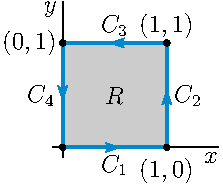
\includegraphics[scale=1.0]
                                        {domainSquare.pdf}}}\\
&\text{$C_2$ from $(1,0)$ to $(1,1)$} \\
&\text{$C_3$ from $(1,1)$ to $(0,1)$} \\
&\text{$C_4$ from $(0,1)$ to $(0,0)$} 
\\[-0.1in]
\end{align*}
Now $x$ is constant on $C_2$ and $C_4$ so that 
\begin{equation*}
\int_{C_2}f(x,y)\,\dee{x} = \int_{C_4}f(x,y)\,\dee{x} =0
\end{equation*}
So, using $-C_3$ to denote the line segment from $(0,1)$ to $(1,1)$
\begin{align*}
\dblInt_R\frac{\partial f}{\partial y}(x,y)\ \dee{x}\,\dee{y}
&=-\left[\int_{C_1}f(x,y)\,\dee{x}+\int_{C_3}f(x,y)\,\dee{x}\right]\\
&=\int_{-C_3}f(x,y)\,\dee{x}-\int_{C_1}f(x,y)\,\dee{x} \\
&=\int_0^1 f(x,1)\ \dee{x}  - \int_0^1 f(x,0)\ \dee{x}
\end{align*}

\end{solution}

%%%%%%%%%%%%%%%%%%%%%%%%%%%%%%%
\begin{question}
 Let $R$ be a finite region in the $xy$-plane,
whose boundary, $C$, consists of a single, piecewise smooth, simple
closed curve that is oriented counterclockwise.
``Simple'' means that the curve does not intersect itself.
Use Green's theorem to show that 
\begin{equation*}
\dblInt_R\vnabla\cdot\vF\ \dee{x}\,\dee{y}=\oint_C\vF\cdot\hn\,\dee{s}
\end{equation*}
where $\vF=F_1\,\hi+F_2\,\hj$, $\hn$ is the outward unit normal to $C$ and $s$ 
is the arclength along $C$.
\begin{center}
       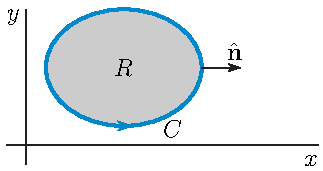
\includegraphics{GreenDiv.pdf}
\end{center}

\end{question}

\begin{hint} 
Let $\vr(s)=x(s)\,\hi+y(s)\,\hj$ be a counterclockwise parametrization of 
$C$ by arc length. Then $\hT(s) = \vr'(s) = x'(s)\,\hi+y'(s)\,\hj$
is the forward pointing unit tangent vector to $C$ at $\vr(s)$
and $\hn(s) = \vr'(s)\times\hk=y'(s)\,\hi-x'(s)\,\hj$. To see
that $\vr'(s)\times\hk$ really is $\hn(s)$, note that 
$y'(s)\,\hi-x'(s)\,\hj$ 
\begin{itemize}\itemsep1pt \parskip0pt \parsep0pt
\item
has the same length, namely $1$, as $\vr'(s)$ (recall that $\vr(s)$ is a
parametrization by arc length),
\item
lies in the $xy$-plane and 

\item
is perpendicular to $\vr'(s)$. 
(Check that $\vr'(s)\cdot\big[y'(s)\,\hi-x'(s)\,\hj\big]=0$.) 
\item
Use the right hand rule to check that $\vr'(s)\times\hk$ is 
$\hn$ rather than $-\hn$.
\end{itemize}
\end{hint}

\begin{answer} 
See the solution.
\end{answer}

\begin{solution} 
Let $\vr(s)=x(s)\,\hi+y(s)\,\hj$ be a counterclockwise parametrization of 
$C$ by arc length. Then $\hT(s) = \vr'(s) = x'(s)\,\hi+y'(s)\,\hj$
is the forward pointing unit tangent vector to $C$ at $\vr(s)$
and $\hn(s) = \vr'(s)\times\hk=y'(s)\,\hi-x'(s)\,\hj$. To see
that $\vr'(s)\times\hk$ really is $\hn(s)$, note that 
$y'(s)\,\hi-x'(s)\,\hj$ 
\begin{itemize}\itemsep1pt \parskip0pt \parsep0pt
\item
has the same length, namely $1$, as $\vr'(s)$ (recall that $\vr(s)$ is a
parametrization by arc length),
\item
lies in the $xy$-plane and 

\item
is perpendicular to $\vr'(s)$. 
(Check that $\vr'(s)\cdot\big[y'(s)\,\hi-x'(s)\,\hj\big]=0$.) 
\item
Use the right hand rule to check that $\vr'(s)\times\hk$ is 
$\hn$ rather than $-\hn$.
\end{itemize}
\begin{center}
       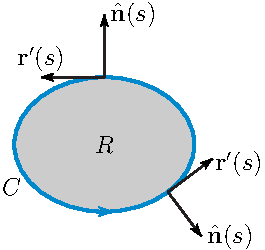
\includegraphics{GreenDivB.pdf}
\end{center}
So, by Green's theorem,
\begin{align*}
\oint_C\vF\cdot\hn\,\dee{s}
&=\oint_C\left[F_1\,\diff{y}{s}-F_2\,\diff{x}{s}\right]\,\dee{s}
=\oint_C\left[-F_2\,\dee{x}+F_1\,\dee{y}\right]
=\dblInt_R\left[\pdiff{}{x}F_1-\pdiff{}{y}(-F_2)\right]\ \dee{x}\,\dee{y} \\
&=\dblInt_R\vnabla\cdot\vF\ \dee{x}\,\dee{y}
\end{align*}
\end{solution}


%%%%%%%%%%%%%%%%%%%%%%%%%%%%%%%
\begin{question}\label{prb Green singular}
Integrate $\dst\frac{1}{2\pi}\oint_C \frac{x\,\dee{y}-y\,\dee{x}}{x^2+y^2}$
counterclockwise around 
\begin{enumerate}[(a)]
\item the circle $x^2+y^2=a^2$
\item the boundary of the square with vertices
         $(-1,-1)$, $(-1,1)$, $(1,1)$ and $(1,-1)$ 
\item the boundary of the region $1\le x^2+y^2\le 2,\ y\ge0$ 
\end{enumerate}
\end{question}

\begin{hint} 
Use direct evaluation!
\end{hint}

\begin{answer}
(a) $1$ \qquad
(b) $1$ \qquad
(c) $0$
\end{answer}

\begin{solution} 
(a) Parametrize the circle by 
$x=a\cos\theta,\ y=a\sin\theta$, $0\le\theta\le 2\pi$. Then
$\dee{x}=-a\sin\theta\,\dee{\theta}$ and 
$\dee{y}=a\cos\theta\,\dee{\theta}$ so that
\begin{align*}
\frac{1}{2\pi}\oint_C \frac{x\,\dee{y}-y\,\dee{x}}{x^2+y^2}
=\frac{1}{2\pi}\int_0^{2\pi} \frac{a^2\cos^2\theta\,\dee{\theta}+a^2\sin^2\theta\,\dee{\theta}}
             {a^2\cos^2\theta+a^2\sin^2\theta}
=\frac{1}{2\pi}\int_0^{2\pi}\dee{\theta}=1
\end{align*}

(b) The boundary of the square has four sides --- one
with $y=-1$, one with $x=1$, one with $y=1$ and one with $x=-1$.
\begin{center}
       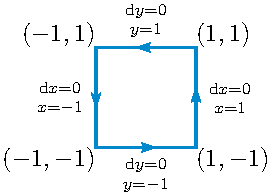
\includegraphics{singGnA.pdf}
\end{center}
To evaluate the integrals over the four sides
\begin{itemize}\itemsep1pt \parskip0pt \parsep0pt %\itemindent-15pt
\item[$\circ$] 
parametrize the $y=-1$ part by $x$ so that
$\vr(x)  = x\,\hi-\hj$, $\vr'(x)=\hi$, with $x$ running from $-1$ to $1$,
\item[$\circ$] 
parametrize the $x=+1$ part by $y$ so that
$\vr(y)  = \hi+y\,\hj$, $\vr'(y)=\hj$, with $y$ running from $-1$ to $1$,
\item[$\circ$] 
parametrize the $y=+1$ part by $x$ so that
$\vr(x)  = x\,\hi+\hj$, $\vr'(x)=\hi$, with $x$ running from $1$ to $-1$, and
\item[$\circ$] 
parametrize the $x=-1$ part by $y$ so that
$\vr(y)  = -\hi+y\,\hj$, $\vr'(y)=\hj$, with $y$ running from $1$ to $-1$,
\end{itemize}
so that the integral
\begin{align*}
\frac{1}{2\pi}\oint_C \frac{x\,\dee{y}-y\,\dee{x}}{x^2+y^2}
&=\frac{1}{2\pi}\overbrace{\int_{-1}^1 \frac{-(-1)\dee{x}}{x^2+1}}^{y=-1{\rm\ part}}
+\frac{1}{2\pi}\overbrace{\int_{-1}^1 \frac{(1)\dee{y}}{1+y^2}}^{x=+1{\rm\ part}}
+\frac{1}{2\pi}\overbrace{\int^{-1}_1 \frac{-(1)\dee{x}}{x^2+1}}^{y=+1{\rm\ part}}
+\frac{1}{2\pi}\overbrace{\int^{-1}_1 \frac{(-1)\dee{y}}{1+y^2}}^{x=-1{\rm\ part}}
\\
&=4\frac{1}{2\pi}\arctan x\bigg|_{-1}^1
=\frac{2}{\pi}\Big[\frac{\pi}{4}+\frac{\pi}{4}\Big]
=1
\end{align*}

(c)
As in part (a) with $a=\sqrt{2}$, but with $\theta$ running from $0$ to $\pi$, 
the outer semicircle gives 
\begin{equation*}
\frac{1}{2\pi}\int_0^{\pi} \frac{a^2\cos^2\theta\,\dee{\theta}+a^2\sin^2\theta\,\dee{\theta}}
             {a^2\cos^2\theta+a^2\sin^2\theta}
=\frac{1}{2\pi}\int_0^{\pi}\dee{\theta}
=\frac{1}{2}
\end{equation*}
\begin{center}
       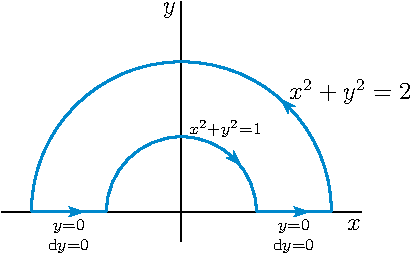
\includegraphics{singGnB.pdf}
\end{center}
As in part (a) with $a=1$, but with $\theta$ running from $\pi$ to $0$, 
the inner semicircle
gives 
\begin{equation*}
\frac{1}{2\pi}\int^0_{\pi} \frac{a^2\cos^2\theta\,\dee{\theta}+a^2\sin^2\theta\,\dee{\theta}}
             {a^2\cos^2\theta+a^2\sin^2\theta}
=\frac{1}{2\pi}\int^0_{\pi}\dee{\theta}
=-\frac{1}{2}
\end{equation*}
The two flat pieces each give zero, since
on them $y=0$ and $\dee{y}=0$. So 
\begin{equation*}
\frac{1}{2\pi}\oint_C \frac{x\,\dee{y}-y\,\dee{x}}{x^2+y^2}
=\frac{1}{2}+0-\frac{1}{2}+0=0
\end{equation*}


\end{solution}

%%%%%%%%%%%%%%%%%%%%%%%%%%%%%%%
\begin{question}
Show that
\begin{align*}
\pdiff{}{x}\Big( \frac{x}{x^2+y^2}\Big)
=\pdiff{}{y}\Big( \frac{-y}{x^2+y^2}\Big)
\end{align*}
for all $(x,y)\ne (0,0)$. Discuss the connection between this result and
the results of Q[\ref{prb Green singular}].
\end{question}

\begin{hint} 
The functions $\frac{x}{x^2+y^2}$
and $\frac{-y}{x^2+y^2}$ are not defined, let alone continuous or
differentiable, at $x=y=0$.
\end{hint}

\begin{answer} 
See the solution.
\end{answer}

\begin{solution} 
The two partial derivatives
\begin{alignat*}{3}
\pdiff{}{x}\Big( \frac{x}{x^2+y^2}\Big)
&=\ \ \frac{(x^2+y^2)-x(2x)}{{(x^2+y^2)}^2}
&&=\frac{y^2-x^2}{{(x^2+y^2)}^2}\\
\pdiff{}{y}\Big( \frac{-y}{x^2+y^2}\Big)
&=\frac{-(x^2+y^2)-(-y)(2y)}{{(x^2+y^2)}^2}
&&=\frac{y^2-x^2}{{(x^2+y^2)}^2}\\
\end{alignat*}
are well-defined and equal everywhere except at the origin $(0,0)$.

\emph{Short discussion:}\ \ \ 
Were it not for the singularity at $(0,0)$, the vector field of the last
problem would be conservative and the integral $\int\vF\cdot \dee{\vr}$
around any closed curve would be zero. But as we saw in parts (a) and (b) of
Q[\ref{prb Green singular}], this is not the case. On the other hand, 
by Green's theorem  (Theorem \eref{CLP317}{thm:Green} in the CLP-4 text), 
the integral around the boundary of any region that
does not contain $(0,0)$ is zero, as happened in part (c) of 
Q[\ref{prb Green singular}]. 

\emph{Long discussion:}\ \ \ First consider part (c) of
Q[\ref{prb Green singular}]. The curve $C$ is the boundary of 
the region
\begin{equation*}
R = \Set{(x,y)}{1\le x^2+y^2\le 2,\ y\ge 0}
\end{equation*}
The partial derivatives 
$\pdiff{}{x}\Big( \frac{x}{x^2+y^2}\Big)$
and
$\pdiff{}{y}\Big( \frac{-y}{x^2+y^2}\Big)$
are well-defined and equal everywhere in $R$. So by Green's
theorem
\begin{equation*}
\frac{1}{2\pi}\oint_C \frac{x\,\dee{y}-y\,\dee{x}}{x^2+y^2}
=\frac{1}{2\pi}\dblInt_R\left[
   \pdiff{}{x}\Big( \frac{x}{x^2+y^2}\Big)
 -\pdiff{}{y}\Big( \frac{-y}{x^2+y^2}\Big)\right]\dee{x}\, \dee{y} 
=0
\end{equation*}
which is the answer we got before. 

We cannot apply Green's theorem
in this way for parts (a) and (b) of Q[\ref{prb Green singular}] because
the singularity at $(0,0)$ is inside the curve $C$ for both parts 
(a) and (b). On the other hand suppose, for simplicity, that $0<a<1$. 
Denote by $C_a$, $C_b$ the curves of parts (a) and (b),
respectively. Define $R$ to be the set of points that are inside $C_b$  
and outside $C_a$. That is,
\begin{equation*}
R=\Set{(x,y)}{-1\le x \le 1,\ -1\le y\le 1,\ x^2+y^2\ge a^2 }
\end{equation*}
Then the boundary, $\partial R$, of $R$ consists of two parts. 
One part is $C_b$.
The other part is $C_a$, but oriented clockwise rather than
counterclockwise. We'll call it $-C_a$.
\begin{center}
       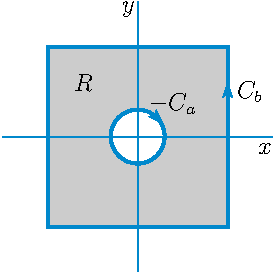
\includegraphics{singGnC.pdf}
\end{center}
Again the partial derivatives 
$\pdiff{}{x}\Big( \frac{x}{x^2+y^2}\Big)$
and
$\pdiff{}{y}\Big( \frac{-y}{x^2+y^2}\Big)$
are well-defined and equal everywhere in $R$. So by Green's theorem
\begin{equation*}
\frac{1}{2\pi}\oint_{\partial R} \frac{x\,\dee{y}-y\,\dee{x}}{x^2+y^2}
=\frac{1}{2\pi}\dblInt_R\left[
   \pdiff{}{x}\Big( \frac{x}{x^2+y^2}\Big)
 -\pdiff{}{y}\Big( \frac{-y}{x^2+y^2}\Big)\right]\dee{x}\, \dee{y} 
=0
\end{equation*}
Consequently
\begin{align*}
0 &= \frac{1}{2\pi}\oint_{\partial R} \frac{x\,\dee{y}-y\,\dee{x}}{x^2+y^2}
= \frac{1}{2\pi}\oint_{C_b} \frac{x\,\dee{y}-y\,\dee{x}}{x^2+y^2}
+ \frac{1}{2\pi}\oint_{-C_a} \frac{x\,\dee{y}-y\,\dee{x}}{x^2+y^2}
\\
&=\frac{1}{2\pi}\oint_{C_b} \frac{x\,\dee{y}-y\,\dee{x}}{x^2+y^2}
- \frac{1}{2\pi}\oint_{C_a} \frac{x\,\dee{y}-y\,\dee{x}}{x^2+y^2}
\end{align*} 
and we conclude that the answers to parts (a) and (b) should be
the same.We did indeed see that in Q[\ref{prb Green singular}].
\end{solution}



%%%%%%%%%%%%%%%%%%
\subsection*{\Procedural}
%%%%%%%%%%%%%%%%%%

%%%%%%%%%%%%%%%%%%%%%%%%%%%
\begin{question}
Evaluate   $\int_C\vF\cdot d\vr$ where 
$\vF = x^2y^2\,\hi + 2xy\,\hj$ and $C$ is the boundary of the square in the 
$xy$-plane having one vertex at the origin and diagonally opposite vertex at the point $(3, 3)$, oriented counterclockwise.
\end{question}

\begin{hint} 
For practice, evaluate this integral twice --- once directly and once
using Green's theorem.
\end{hint}

\begin{answer} 
$-54$
\end{answer}


\begin{solution}
\emph{Solution 1 (direct evaluation)}:\ \ \ 
Here is a sketch of $C$.
\begin{center}
     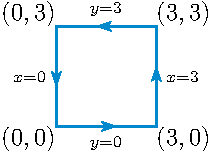
\includegraphics{square3.pdf}
\end{center}
The square consists of four line segments.
\begin{itemize}\itemsep1pt \parskip0pt \parsep0pt %\itemindent-15pt
\item
The bottom line segment may be parametrized
$\vr(x)=(x,0),\ 0\le x\le 3$. So the line integral along
this segment is
\begin{equation*}
\int_0^3 \vF(\vr(x))\cdot\diff{\vr}{x}\ \dee{x}
=\int_0^3 (0, 0)\cdot(1, 0)\ \dee{x}
=0
\end{equation*}
\item
The second line segment may be parametrized
$\vr(y)=(3,y),\ 0\le y\le 3$. So the line integral along
this segment is
\begin{equation*}
\int_0^3 \vF(\vr(y))\cdot\diff{\vr}{y}\ \dee{y}
=\int_0^3 (9y^2, 6y)\cdot(0, 1)\ \dee{y}
=\int_0^3 6y\ \dee{y}
=27
\end{equation*}
\item
The third line segment may be parametrized
$\vr(t)=(3-t,3),\ 0\le t\le 3$. So the line integral along
this segment is
\begin{equation*}
\int_0^3 \vF(\vr(t))\cdot\diff{\vr}{t}\ \dee{t}
=\int_0^3 \big(9(3-t)^2\,,\, 6(3-t)\big)\cdot(-1\,,\,0)\ \dee{t}
=-\int_0^3 9(3-t)^2\ \dee{t}
=-81
\end{equation*}
\item
The final line segment may be parametrized
$\vr(t)=(0,3-t),\ 0\le t\le 3$. So the line integral along
this segment is
\begin{equation*}
\int_0^3 \vF(\vr(t))\cdot\diff{\vr}{t}\ \dee{t}
=\int_0^3 (0, 0)\cdot(0, -1)\ \dee{t}
=0
\end{equation*}
\end{itemize}
The full line integral is
\begin{equation*}
\oint_C\vF\cdot d\vr=0+27-81+0=-54
\end{equation*}


\emph{Solution 2 (Green's theorem)}:\ \ \ 
 We apply Green's Theorem. 
\begin{align*}
\oint_C x^2y^2\,\dee{x}+2xy\,\dee{y}
&=\int_0^3\dee{x}\int_0^3 \dee{y}\ 
            \left[\pdiff{}{x}(2xy)-\pdiff{}{y}(x^2y^2)\right]\\
&=\int_0^3\dee{x}\int_0^3 \dee{y}\ \big[2y-2x^2y\big]\\
&=\int_0^3\dee{x}\ \big[9-9x^2\big]\\
&=27-9\frac{3^3}{3}=-54
\end{align*}
\end{solution}



%%%%%%%%%%%%%%%%%%%%%%%%%%%%%%%
\begin{question}
Evaluate
 $\dst\oint_C (x\sin y^2 -y^2)\,\dee{x}+(x^2y\cos y^2+3x)\,\dee{y}$ 
where $C$ is the
counterclockwise boundary of the trapezoid with vertices $(0,-2),\ (1,-1),\
(1,1)$ and $(0,2)$.
\end{question}

\begin{hint} 
The $\sin y^2$ and $\cos y^2$ in the integrand look hard to integrate.
Try Green's theorem.
\end{hint}

\begin{answer} 
$9$
\end{answer}

\begin{solution} 
Call the trapezoid $T$. 
\begin{center}
       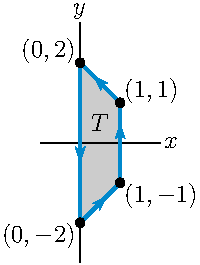
\includegraphics{trapGn.pdf}
\end{center}
By Green's theorem,
\begin{align*}
&\oint_C (x\sin y^2 -y^2)\,\dee{x}+(x^2y\cos y^2+3x)\,\dee{y} \\
&\hskip1in=\dblInt_T\left\{\pdiff{}{x}(x^2y\cos y^2+3x)
-\pdiff{}{y} (x\sin y^2 -y^2)\right\}\,\dee{x}\,\dee{y}\\
&\hskip1in=\dblInt_T\big(2xy\cos y^2+3-2xy\cos y^2+2y\big)\,\dee{x}\,\dee{y}\\
&\hskip1in=\dblInt_T\big(3+2y\big)\,\dee{x}\,\dee{y}
\end{align*}
The integral $\dblInt_T(2y)\,\dee{x}\,\dee{y}$ vanishes because $2y$ changes
sign under $y\rightarrow-y$ while the domain of 
integration is invariant under $y\rightarrow -y$.  The integral 
$\dblInt_T 3\,\dee{x}\,\dee{y}$ is $3$ times the area of the
trapezoid, which is its width (1) times the average of its heights
$(\half[2+4])=3$. So 
\begin{equation*}
\oint_C (x\sin y^2 -y^2)\,\dee{x}+(x^2y\cos y^2+3x)\,\dee{y}
               =3\times 1\times 3 = 9
\end{equation*}
\end{solution}

%%%%%%%%%%%%%%%%%%%%%%%%%%%
\begin{question}[M317 1999A] %4
 Evaluate 
$ I=
\dst\oint_{\cC} \Big(\frac{1}{3}x^2y^3-x^4y\Big)\,\dee{x}
+\big(xy^4+x^3y^2\big)\,\dee{y}
$
counterclockwise around the boundary of the half-disk $0\le y\le \sqrt{4-x^2}$.
\end{question}

\begin{hint} 
Don't do the integral directly. 
\end{hint}

\begin{answer} 
$\frac{32}{3}\pi$
\end{answer}

\begin{solution} 
\emph{(Using Green's theorem:)}\ \ \ 
By Green's theorem  (Theorem \eref{CLP317}{thm:Green} in the CLP-4 text), 
using $D$ to
denote the half-disk $0\le y\le \sqrt{4-x^2}$,
\begin{align*}
&\dst\oint_{\cC} \Big(\frac{1}{3}x^2y^3-x^4y\Big)\,\dee{x}
+\big(xy^4+x^3y^2\big)\,\dee{y}
=\dblInt_D\Big[\pdiff{}{x}\big(xy^4+x^3y^2\big)
-\pdiff{}{y}\Big(\frac{1}{3}x^2y^3-x^4y\Big) \Big] \dee{x} \dee{y}\\
&\hskip1in=\dblInt_D\big(x^4+2x^2y^2+y^4\big)\ \dee{x} \dee{y}
=\dblInt_D\big(x^2+y^2\big)^2\ \dee{x} \dee{y}
\end{align*}
Switching to polar coordinates
\begin{align*}
\dst\oint_{\cC} \Big(\frac{1}{3}x^2y^3-x^4y\Big)\,\dee{x}
+\big(xy^4+x^3y^2\big)\,\dee{y}
&=\int_0^2 dr\ r\int_0^{\pi}\dee{\theta}\ r^4
={\pi\frac{r^6}{6}\bigg|}_0^2
=\frac{32}{3}\pi
\end{align*}

\emph{(Using direct evaluation:)}\ \ \ 
Write $\cC$ as the union of $\cC_1$, the straight line from
$(-2,0)$ to $(2,0)$, and $\cC_2$, the half-circle $\vr(\theta)=x(\theta)\,\hi+y(\theta)\,\hj=2\cos\theta\,\hi+2\sin\theta\,\hj$,
$0\le\theta\le \pi$. As $y=0$ at every point of $\cC_1$,
$\ 
\int_{\cC_1} \big(\frac{1}{3}x^2y^3-x^4y\big)\,\dee{x}
+\big(xy^4+x^3y^2\big)\,\dee{y}=0
\ $ and
\begin{align*}
I&=\int_{\cC_2} \Big(\frac{1}{3}x^2y^3-x^4y\Big)\,\dee{x}
+\big(xy^4+x^3y^2\big)\,\dee{y}\\
&=\int_0^\pi\Big[ \Big(\frac{1}{3}x(\theta)^2y(\theta)^3-x(\theta)^4y(\theta)\Big)\,x'(\theta)
+\big(x(\theta)y(\theta)^4+x(\theta)^3y(\theta)^2\big)y'(\theta)\Big]
          \dee{\theta}
\\
&=\int_0^\pi\Big[ \Big(\frac{1}{3}2^5\cos^2\theta\sin^3\theta-2^5\cos^4\theta\sin\theta\Big)\,
                 (-2\sin\theta)
   \\&\hskip2in
+\big(2^5\cos\theta\sin^4\theta+2^5\cos^3\theta\sin^2\theta\big)\,
               (2\cos\theta)\Big]\dee{\theta}\\
&=2^5\int_0^\pi \Big(\frac{4}{3}\cos^2\theta\sin^4\theta+4\cos^4\theta\sin^2\theta\Big)
\dee{\theta}\\
&=2^5\int_0^\pi \sin^2(2\theta)\big(\frac{1}{3}\sin^2\theta+\cos^2\theta\big)\,
\dee{\theta}\\
&=2^4\int_0^\pi \sin^2(2\theta)\Big(\frac{1}{3}[1-\cos(2\theta)]+[1+\cos(2\theta)]\Big)\,
\dee{\theta}\\
  &\hskip2in\hbox{ since }\cos(2\theta)=2\cos^2\theta-1=1-2\sin^2\theta\\
&=\frac{2^5}{3}\int_0^\pi \sin^2(2\theta)\big[2+\cos(2\theta)\big]\ \dee{\theta}\\
&=\frac{2^5}{3}\int_0^\pi \big[1-\cos(4\theta)+\sin^2(2\theta)\cos(2\theta)\big]\ \dee{\theta}\\
&=\frac{2^5}{3} \Big[\theta-\frac{1}{4}\sin(4\theta)+\frac{1}{6}\sin^3(2\theta)\Big]_0^\pi
=\frac{32}{3}\pi
\end{align*}
\end{solution}


%%%%%%%%%%%%%%%%%%%%%%%%%%%
\begin{question}[M317 2018A] %6
Let $\cC$ be the counterclockwise boundary of the rectangle
with vertices $(1,0)$, $(3,0)$, $(3,1)$ and $(1,1)$. Evaluate
\begin{equation*}
\oint_\cC\big(3y^2+2xe^{y^2}\big)\,\dee{x} + \big(2yx^2 e^{y^2}\big)\,\dee{y}
\end{equation*}
\end{question}

\begin{hint} 
Don't do the integral directly. Sketch the rectangle.
\end{hint}

\begin{answer} 
$-6$
\end{answer}

\begin{solution} 
Let's use Green's theorem. The
rectangle, which we shall denote $\cR$, is
\vskip0.25in
\begin{align*}
\cR=\set{(x,y)}{1\le x\le 3,\ 0\le y\le 1}
\qquad\raisebox{-50pt}[40pt][40pt]{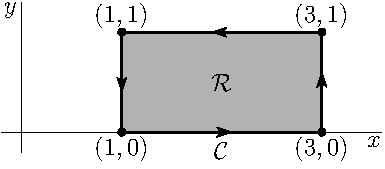
\includegraphics{domainPlgmB.pdf}}
\end{align*}
\vskip0.15in
\item{}So Green's theorem gives
\begin{align*}
\oint_\cC\big(3y^2+2xe^{y^2}\big)\,\dee{x} + \big(2yx^2 e^{y^2}\big)\,\dee{y}
&=\dblInt_\cR \Big[
      \pdiff{}{x}\big(2yx^2 e^{y^2}\big)  
     -\pdiff{}{y}\big(3y^2+2xe^{y^2}\big)  
   \Big]\,\dee{x} \dee{y} \\
&=\dblInt_\cR \Big[
      4xy e^{y^2}
     -6y -4xye^{y^2}
   \Big]\,\dee{x} \dee{y} \\
& = -6 \int_1^3 \dee{x}\int_0^1 \dee{y}\ y 
       = -6 \int_1^3 \dee{x}\ \frac{1}{2} \\
&=-6
\end{align*}
\end{solution}

\begin{question}[M317 2016A] %1
Consider the closed region enclosed by the curves 
$y = x^2 + 4x + 4$ and $y = 4 - x^2$. Let
$C$ be its boundary and suppose that $C$ is oriented counter-clockwise.
\begin{enumerate}[(a)]
\item
   Draw the \emph{oriented} curve $C$ carefully in the $xy$-plane.
\item
    Determine the value of
    \begin{equation*}
         \oint_C xy\, \dee{x} + (e^y + x^2 ) \dee{y}
     \end{equation*}
\end{enumerate}

\end{question}

\begin{hint} 
Do not compute the integral directly.
\end{hint}

\begin{answer}
(a)
\begin{center}
       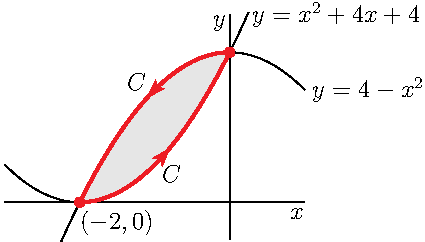
\includegraphics{OE16A_1a.pdf}
\end{center}

 
(b) $-\frac{8}{3}$
\end{answer}

\begin{solution}  (a)
The curves $y = x^2 + 4x + 4$ and $y = 4 - x^2$ meet when
\begin{equation*}
x^2 + 4x + 4 = 4 - x^2
\iff 2x^2  +4x = 2x(x+2) = 0
\end{equation*}
So the curves intersect at $(0,4)$ and  $(-2,0)$. Here is a sketch.
\begin{center}
       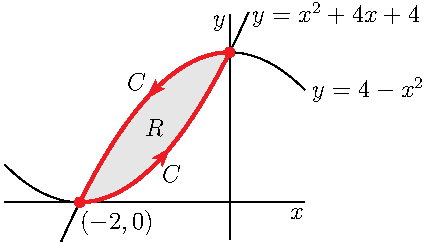
\includegraphics{OE16A_1.pdf}
\end{center}


\noindent (b) Let
\begin{equation*}
R=\Set{(x,y)\in\bbbr^2}{ x^2+4x+4\le y\le  4-x^2,\ -2\le x\le 0}
\end{equation*}
By Green's theorem (Theorem \eref{CLP317}{thm:Green} in the CLP-4 text)
\begin{align*}
\oint_C xy\, \dee{x} + (e^y + x^2 ) \dee{y}
&=\dblInt_R \left\{
  \tfrac{\partial\hfill}{\partial x}(e^y+x^2)
  -\tfrac{\partial\hfill}{\partial y}(xy)
\right\}\dee{x}\dee{y} \\
&= \int_{-2}^0\dee{x} \int_{x^2+4x+4}^{4-x^2}\dee{y} \ x \\
&= \int_{-2}^0\dee{x}\ (-2x^2-4x) x \\
&=\left[-\frac{x^4}{2} -\frac{4x^3}{3}\right]^0_{-2} \\
&=-\frac{8}{3}
\end{align*}
\end{solution}

%%%%%%%%%%%%%%%%%%%%%%%%%%%
\begin{question}[M317 2010D] %4
Let
\begin{equation*}
\vF(x, y) = \big(y^2 - e^{-y^2} + \sin x\,,\, 2xye^{-y^2} + x\big)
\end{equation*}
Let $C$ be the boundary of the triangle with vertices $(0, 0)$, $(1, 0)$ and 
$(1, 2)$, oriented counter-clockwise. Compute
\begin{equation*}
\int_C \vF\cdot\dee{\vr}
\end{equation*}
\end{question}

\begin{hint} 
Don't do the integral directly. Sketch the triangle.
\end{hint}

\begin{answer} 
$-\frac{1}{3}$
\end{answer}

\begin{solution} 
The integral that would be used for direct evaluation looks very
complicated. So let's try Green's theorem. The curve $C$ is the
boundary of the triangle
\begin{equation*}
T = \Set{(x,y)}{0\le x\le 1, 0\le y\le 2x}
\end{equation*}
\begin{center}
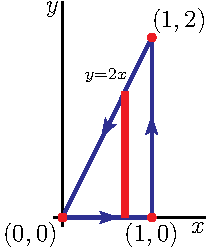
\includegraphics{OE10D_4.pdf}
\end{center}
So
\begin{align*}
\int_C \vF\cdot\dee{\vr}
&= \int_C \big\{\big(y^2 - e^{-y^2} + \sin x\big)\dee{x}
               +\big(2xye^{-y^2} + x\big)\dee{y}\big\} \\
&= \dblInt_T \big\{
             \tfrac{\partial\hfill}{\partial x}\big(2xye^{-y^2} + x\big)
           -\tfrac{\partial\hfill}{\partial y}\big(y^2 - e^{-y^2} + \sin x\big)
               \big\}\dee{x}\dee{y} \hskip0.1in
%\raisebox{-100pt}[0pt][0pt]{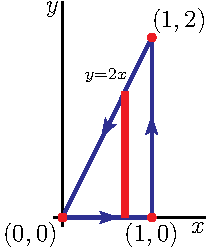
\includegraphics{OE10D_4.pdf}}
\\
&= \dblInt_T \big\{
             \big(2ye^{-y^2} + 1\big)
           - \big(2y +2y e^{-y^2} \big)
               \big\}\dee{x}\dee{y} \\
&= \int_0^1\dee{x}\int_0^{2x}\dee{y}\  \big\{1-2y\big\} \\
&= \int_0^1\dee{x}\  \big\{2x-4x^2\big\} \\
&=1-\frac{4}{3} = -\frac{1}{3}
\end{align*}

\end{solution}

%%%%%%%%%%%%%%%%%%%%%%%%%%%
\begin{question}[M317 2009A] %4
Suppose the curve $C$ is the boundary of the region enclosed between 
the curves $y = x^2 - 4x+3$ and $y = 3 - x^2 + 2x$. Determine the value 
of the line integral
\begin{equation*}
\int_C \big(2xe^y + \sqrt{2 + x^2}\big)\, \dee{x} 
            + x^2 (2 + e^y)\, \dee{y}
\end{equation*}
where $C$ is traversed counter-clockwise.
\end{question}

\begin{hint} 
The integrand for direct evaluation looks complicated ---
don't evaluate this integral directly.
\end{hint}

\begin{answer} 
$54$
\end{answer}

\begin{solution} 
Here is a sketch of the two curves in question.

\begin{center}
       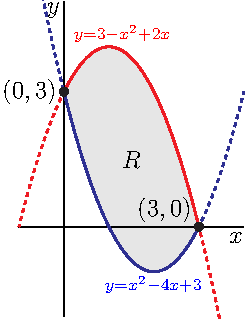
\includegraphics{OE09A_4.pdf}
\end{center}

Note that the curves $y = x^2 - 4x+3$ and $y = 3 - x^2 + 2x$
intersect when $x^2 - 4x+3 = 3 - x^2 + 2x$ or $2x^2-6x=2x(x-3)=0$ or
$x=0$, $3$. 

The integrand for direct evaluation looks complicated. So
let's use Green's theorem with 
$F_1(x,y) = 2xe^y + \sqrt{2 + x^2}$, $F_2(x,y)= x^2 (2 + e^y)$
and 
\begin{equation*}
R=\Set{(x,y)}{x^2 - 4x+3 \le y\le 3 - x^2 + 2x,\ 0\le x\le 3}
\end{equation*}
By Green's theorem, which is Theorem \eref{CLP317}{thm:Green} 
in the CLP-4 text,
\begin{align*}
\int_C \big(2xe^y + \sqrt{2 + x^2}\big)\, \dee{x} 
            + x^2 (2 + e^y)\, \dee{y}
&=\dblInt_R\left\{\frac{\partial F_2}{\partial x}
                 -\frac{\partial F_1}{\partial y}\right\}\ \dee{x}\dee{y} \\
&=\dblInt_R\left\{2x(2+e^y) - 2xe^y\right\}\ \dee{x}\dee{y} \\
&=4 \int_0^3\dee{x} \int_{x^2 - 4x+3}^{3 - x^2 + 2x}\dee{y}\ x \\
&=4 \int_0^3\dee{x}\ (6x-2x^2) x \\
&=4\left[2x^3-\frac{1}{2}x^4\right]_0^3 \\
&=54
\end{align*}


\end{solution}


%%%%%%%%%%%%%%%%%%%%%%%%%%%
\begin{question}[M317 2006A] %4
Let
\begin{align*}
\vF(x,y) = \big(\tfrac{3}{2}y^2 + e^{-y} +\sin x\big)\,\hi
           +\big(\tfrac{1}{2}x^2+x-x e^{-y}\big)\,\hj
\end{align*}
Find $\int_C\vF\cdot\dee{\vr}$, where $C$ is the boundary of the triangle
$(0,0)$, $(1,-2)$, $(1,2)$, oriented anticlockwise.

\end{question}

\begin{hint} 
Direct evaluation is not the most efficient method available.
\end{hint}

\begin{answer} 
$\frac{10}{3}$
\end{answer}

\begin{solution}
Direct evaluation will lead to three integrals, one for each side of the 
triangle. The integral from $(0,0)$ and $(1,-2)$ and the integral from 
$(1,2)$ to $(0,0)$ will each contain six (nonconstant) terms. This 
does not look very efficient.
So let's try Green's theorem. Denote by $T$, the triangle
\begin{equation*}
T = \Set{(x,y)}{0\le x\le 1,\ -2x\le y\le 2x} \hskip0.5in
\raisebox{-50pt}[40pt][40pt]{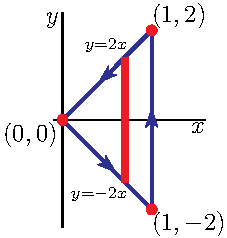
\includegraphics{OE06A_4.pdf}}
\end{equation*}
It has boundary $\partial T=C$, oriented counterclockwise as desired.
So, by Green's theorem,
\begin{align*}
\int_C \vF\cdot\dee{\vr}
&= \int_{\partial T} \big\{\big(\tfrac{3}{2}y^2 + e^{-y} +\sin x\big)\dee{x}
               +\big(\tfrac{1}{2}x^2+x-x e^{-y}\big)\dee{y}\big\} \\
&= \dblInt_T \big\{
    \tfrac{\partial\hfill}{\partial x}\big(\tfrac{1}{2}x^2+x-x e^{-y}\big)
   -\tfrac{\partial\hfill}{\partial y}\big(\tfrac{3}{2}y^2 + e^{-y} +\sin x\big)
               \big\}\dee{x}\dee{y}
\\
&= \dblInt_T \big\{
             \big(x + 1-e^{-y}\big)
           - \big(3y - e^{-y} \big)
               \big\}\dee{x}\dee{y} \\
&= \dblInt_T \big\{ x -3y + 1 \big\}\dee{x}\dee{y} 
\end{align*}
Now 
\begin{align*}
\dblInt_T  \dee{x}\dee{y} &=\text{Area}(T) = \frac{1}{2}(4)(1) = 2 \\
\dblInt_T  y\ \dee{x}\dee{y} &= 0
   \qquad\text{since $y$ is odd under $y\rightarrow-y$} \\
\dblInt_T  x\ \dee{x}\dee{y} 
&=\int_0^1\dee{x}\int_{-2x}^{2x} \dee{y}\ x
 =\int_0^1 4x^2\ \dee{x} 
 =\frac{4}{3}
\end{align*}
So
\begin{equation*}
\int_C \vF\cdot\dee{\vr} = \frac{4}{3}-3\times 0 +2 =\frac{10}{3}
\end{equation*}
\end{solution}

%%%%%%%%%%%%%%%%%%%%%%%%%%%%%%%%%%%%%%%%%%%%
\begin{question}[M317 2015A]  %4
\begin{enumerate}[(a)]
\item
Use Green's theorem to evaluate the line integral
\begin{equation*}
\int_C \frac{-y}{x^2+y^2}\dee{x} + \frac{x}{x^2+y^2}\dee{y}
\end{equation*}
where $C$ is the arc of the parabola $y = \frac{1}{4}x^2 + 1$ from 
$(-2, 2)$ to $(2, 2)$. 


\item
Use Green's theorem to evaluate the line integral
\begin{equation*}
\int_C \frac{-y}{x^2+y^2}\dee{x} + \frac{x}{x^2+y^2}\dee{y}
\end{equation*}
where $C$ is the arc of the parabola $y = x^2 -2$ from 
$(-2, 2)$ to $(2, 2)$.


\item
Is the vector field
\begin{equation*}
\vF=\frac{-y}{x^2+y^2}\hi + \frac{x}{x^2+y^2}\hj
\end{equation*}
conservative? Provide a reason for your answer based on your answers 
to the previous parts of this question.
\end{enumerate}

\end{question}

\begin{hint} 
Green's theorem must be applied to a closed curve; note that the 
curve $C$ is not closed. 

Consider carefully the point $(0, 0)$ in your analysis. 

You may use the fact that
$\int \frac{\dee{t}}{1+t^2} = \arctan(t) + C$.
\end{hint}

\begin{answer} 
(a) $-\frac{\pi}{2}$\qquad
(b) $\frac{3\pi}{2}$\qquad
(c) No.
\end{answer}

\begin{solution} 
Set
\begin{equation*}
\vF=\frac{-y}{x^2+y^2}\hi + \frac{x}{x^2+y^2}\hj
\end{equation*}

(a) Green's theorem must be applied to a curve that is closed,
so that it is the boundary of a region in $\bbbr^2$. The given curve $C$
is not closed. But it is  part of the boundary of 
\begin{equation*}
R = \Set{(x,y)}{-2\le x\le 2,\ \tfrac{x^2}{4}+1\le y\le 2}
\end{equation*}
Here is a sketch of $R$.
 \begin{center}
    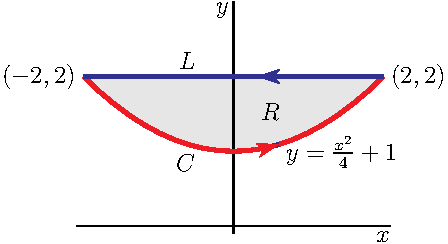
\includegraphics{OE15A_3.pdf}
\end{center}

The boundary of $R$ consists of two parts --- $C$ on the bottom
and the line segment $L$ from $(2,2)$ to $(-2,2)$ on the top.
Note that $\vF$ is well-defined on all of $R$ and that
\begin{align*}
\pdiff{}{x} \vF_2 - 
\pdiff{}{y} \vF_1 
&=\pdiff{}{x} \frac{x}{x^2+y^2} +
\pdiff{}{y} \frac{y}{x^2+y^2} \\
&=\frac{(x^2+y^2) - x(2x)}{{(x^2+y^2)}^2}
  +\frac{(x^2+y^2) - y(2y)}{{(x^2+y^2)}^2} \\
&=0
\end{align*}
on all of $R$. So, by Green's theorem (Theorem \eref{CLP317}{thm:Green} in the CLP-4 text), 
\begin{align*}
\int_C \frac{-y}{x^2+y^2}\dee{x} + \frac{x}{x^2+y^2}\dee{y}
&=\dblInt_R \Big(\pdiff{}{x} \vF_2 - 
          \pdiff{}{y} \vF_1 \Big)\dee{x}\dee{y}
 - \int_L\vF\cdot\dee{\vr} \\
&=\int_{-L}\vF\cdot\dee{\vr} 
  =\int_{-2}^2 \vF_1\,\dee{x}
  =-\int_{-2}^2\frac{2}{x^2+4} \,\dee{x}\quad\text{since $y=2$ on $L$} \\
&=-\int_{-1}^1\frac{4}{4u^2+4} \,\dee{x}
\qquad\text{with $x=2u$, $\dee{x}=2\dee{u}$} \\
&=-\arctan u\Big|_{-1}^1 =-\frac{\pi}{2}
\end{align*}
In the second line, we used the notation $-L$ for the line segment
from $(-2,2)$ to $(2,2)$.

(b) This question looks a lot like that of part (a). But there is
a critical difference. Again $C$ is not closed and again it is
part of the boundary of a simple region in the $xy$-plane, namely
\begin{equation*}
R = \Set{(x,y)}{-2\le x\le 2,\ x^2-2\le y\le 2}
\end{equation*}
This $R$ is sketched below.
 \begin{center}
    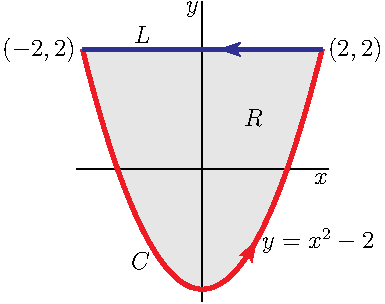
\includegraphics[scale=0.85]{OE15A_3b1.pdf}
\end{center}
We \emph{cannot} continue as in part (a), using this $R$, because 
$\pdiff{}{x} \vF_2 - 
\pdiff{}{y} \vF_1 $ is \emph{not} zero througout $R$.
In fact, it is \emph{not} even defined throughout $R$ --- it is not defined
at $(0,0)$, which is a point of $R$. We can work around this obstruction
by 
\begin{itemize}\itemsep1pt \parskip0pt \parsep0pt %\itemindent-15pt
\item[$\circ$]
choosing a number $\rho>0$ that is small enough that the circle
$C_\rho$ parametrized by
\begin{equation*}
\vr(\theta) = \rho\cos\theta\,\hi +\rho\sin\theta\,\hj\qquad
0\le \theta \le 2\pi
\end{equation*}
is completely contained inside $R$ (ror example, $\rho=1$ is fine)
\item[$\circ$]
and then removing from $R$ the interior of $C_\rho$. 
\end{itemize}
This produces the ``deformed washer''
\begin{equation*}
W = \Set{(x,y)}{-2\le x\le 2,\ x^2-2\le y\le 2,\ x^2+y^2\ge\rho^2}
\end{equation*}
that is sketched below.
 \begin{center}
    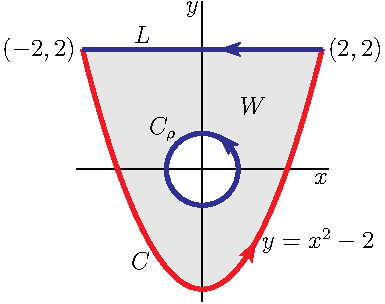
\includegraphics{OE15A_3b2.pdf}
\end{center}
The boundary of $W$ consists the three parts ---
 the curve of interest $C$ on the bottom, 
 the line segment $L$ from $(2,2)$ to $(-2,2)$ on the top,
 and the circle $-C_\rho$ (that is $C_\rho$ but oriented clockwise,
 rather than counter-clockwise) around the hole in the middle. Now 
$\pdiff{}{x} \vF_2 - 
\pdiff{}{y} \vF_1 $
is well-defined and zero throughout $W$. So, by Green's theorem 
(Theorem \eref{CLP317}{thm:Green} in the CLP-4 text), 
\begin{align*}
\int_C \frac{-y}{x^2+y^2}\dee{x} + \frac{x}{x^2+y^2}\dee{y}
&=\dblInt_W \Big(\pdiff{}{x} \vF_2 - 
          \pdiff{}{y} \vF_1 \Big)\dee{x}\dee{y}
 - \int_L\vF\cdot\dee{\vr}- \int_{-C_\rho}\vF\cdot\dee{\vr} \\
&=\int_{-L}\vF\cdot\dee{\vr} 
  + \int_{C_\rho}\vF\cdot\dee{\vr} 
\end{align*}
We have already found, in part (a), that 
$\int_{-L}\vF\cdot\dee{\vr}=-\frac{\pi}{2}$. So it remains only to use
\begin{align*}
\vr(\theta) &= \rho\cos\theta\,\hi +\rho\sin\theta\,\hj \\
\vr'(\theta) &= -\rho\sin\theta\,\hi +\rho\cos\theta\,\hj
\end{align*}
to evaluate
\begin{align*}
\int_{C_\rho}\vF\cdot\dee{\vr}
&=\int_0^{2\pi} \vF\big(\vr(\theta)\big)\cdot\vr'(\theta)\,\dee{\theta} \\
&= \int_0^{2\pi} \Big(\overbrace{-\frac{1}{\rho}\sin\theta\,\hi+\frac{1}{\rho}\cos\theta\,\hj}^
               {\vF(\vr(\theta))}\Big)
 \cdot\big(\overbrace{-\rho\sin\theta\,\hi +\rho\cos\theta\,\hj}^
                     {\vr'(\theta)}\big)\,\dee{\theta} 
=\int_0^{2\pi}\dee{\theta} \\
&=2\pi 
\end{align*}
All together
\begin{equation*}
\int_C \frac{-y}{x^2+y^2}\dee{x} + \frac{x}{x^2+y^2}\dee{y}
=\int_{-L}\vF\cdot\dee{\vr} 
  + \int_{C_\rho}\vF\cdot\dee{\vr} 
=-\frac{\pi}{2} +2\pi
=\frac{3\pi}{2}
\end{equation*}

(c) No, $\vF$ is not conservative. We found, in parts (a) and (b),
two different values for the integrals along two paths, both of which start
at $(-2,2)$ and end at $(2,2)$. So $\vF$ does not have the
``path independence'' property of Theorem \eref{CLP317}{thm:pathIndepConserv}.c
in the CLP-4 text and cannot be conservative.
\end{solution}

%%%%%%%%%%%%%%%%%%%%%%%%%%%%%%%
\begin{question}[M317 2012J] %7
Suppose the curve $C$ is the boundary of the region enclosed between 
the curves $y = x^2 - 4x + 3$ and $y = 3 - x^2 + 2x$. Determine the 
value of the line integral
\begin{equation*}
\int_C \big(2xe^y + \sqrt{2} + x^2\big)\dee{x} 
      + x^2 \big(2 + e^y)\dee{y}
\end{equation*}
where $C$ is traversed counter-clockwise.
\end{question}

\begin{hint} 
If we were to try to evaluate this integral directly, then on the
$y=x^2-4x+3$ part of $C$, the 
integrand would contain $x^2 e^y = x^2 e^{x^2-4x+3}$. That looks hard to integrate, so try Green's theorem. 
\end{hint}

\begin{answer} 
$54$
\end{answer}

\begin{solution}
The given integral is of the form $\int_C \vF\cdot\dee{\vr}$
with
\begin{equation*}
\vF = \big(2xe^y + \sqrt{2} + x^2\big)\,\hi 
      + x^2 \big(2 + e^y)\,\hj
\end{equation*}
If we were to try to evaluate this integral directly, then on the
$y=x^2-4x+3$ part of $C$, the 
integrand would contain $x^2 e^y = x^2 e^{x^2-4x+3}$. That looks hard to integrate, so let's try Green's theorem. 
The parabolas $y = x^2 - 4x + 3$ and $y = 3 - x^2 + 2x$
intersect at $(x,y)$ with
\begin{align*}
x^2 - 4x + 3 = 3 - x^2 + 2x
&\iff
2x^2 -6x = 0
\iff
2x(x-3)=0 \\
&\iff
x=0\text{ or }x=3
\end{align*}
The curve $C$ is the boundary
of 
\begin{equation*}
R= \Set{(x,y)}{0\le x\le 3,\ x^2 - 4x + 3 \le y\le  3 - x^2 + 2x}
\end{equation*}
It is sketched below.
\begin{center}
     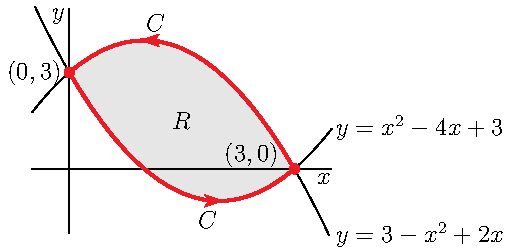
\includegraphics[scale=0.90]{OE12J_7.pdf}
\end{center}
By Green's theorem  (Theorem \eref{CLP317}{thm:Green} in the CLP-4 text), 
\begin{align*}
&\int_C \big(2xe^y + \sqrt{2} + x^2\big)\dee{x} 
      + x^2 \big(2 + e^y)\dee{y} \\
&\hskip1in
= \dblInt_R\Big[\pdiff{}{x}\big(x^2 \big(2 + e^y)\big)
-\pdiff{}{y}\big(2xe^y + \sqrt{2} + x^2\big)\Big] \dee{x}\dee{y}
\\
&\hskip1in = \dblInt_R \big(2x(2+e^y) - 2xe^y\big)\,\dee{x}\dee{y} \\
&\hskip1in =4 \int_0^3\dee{x}\int_{x^2 - 4x + 3}^{3 - x^2 + 2x}\dee{y}\  x 
=4 \int_0^3\dee{x}\ x\big[(3 - x^2 + 2x) - (x^2 - 4x + 3)\big]\\
&\hskip1in =4 \int_0^3\dee{x}\ \big(6x^2-2x^3\big)
= 4\big(2\times 3^3-\frac{1}{2}3^4\big)
=54
\end{align*}
\end{solution}

%%%%%%%%%%%%%%%%%%%%%%%%%%%%%%%
\begin{question}[M317 2016D] %4
Let $\vF(x, y) = P \,\hi + Q\,\hj$ be a smooth plane vector field 
defined for $(x,y) \ne (0, 0)$, and suppose $Q_x = P_y$ for 
$(x,y) \ne  (0, 0)$. In the following $I_j = \int_{C_j} \vF\cdot\dee{\vr}$
for integer $j$, and all $C_j$ are positively oriented circles. Suppose 
$I_1 = \pi$ where $C_1$ is the circle $x^2 + y^2 = 1$.
\begin{enumerate}[(a)]
\item
Find $I_2$ for $C_2 : (x - 2)^2 + y^2 = 1$. Explain briefly.
\item
Find $I_3$ for $C_3 : (x - 2)^2 + y^2 = 9$. Explain briefly.
\item
Find $I_4$ for $C_4 : (x - 2)^2 + (y-2)^2 = 9$. Explain briefly.
\end{enumerate}
\end{question}

\begin{hint} 
Beware the point $(0,0)$.
\end{hint}

\begin{answer} 
(a) $I_2=0$\qquad
(b) $I_3=\pi$\qquad
(c) $I_4=\pi$
\end{answer}

\begin{solution} (a) Denote by
\begin{equation*}
R_2=\Set{(x,y)}{ (x-2)^2+y^2\le 1}
\end{equation*}
the interior of the circle $C_2$. Note that $(0,0)$ is \emph{not}
in $R_2$. Consequently, $Q_x-P_y=0$ \emph{everywhere} in $R_2$ and,
by Green's theorem (Theorem \eref{CLP317}{thm:Green} in the CLP-4 text),
\begin{equation*}
I_2 = \int_{C_2} \vF\cdot\dee{\vr}
    =\dblInt_{R_2} \big(Q_x-P_y\big)\,\dee{x}\dee{y}
    =0
\end{equation*}

\begin{center}
     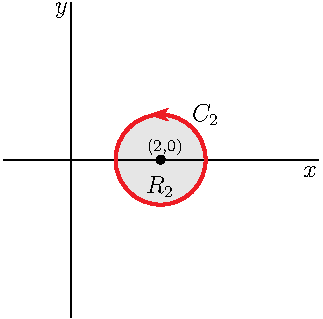
\includegraphics[scale=0.90]{OE16D_4a.pdf}\qquad
     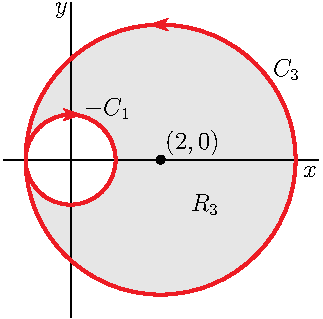
\includegraphics[scale=0.90]{OE16D_4b.pdf}\qquad
%     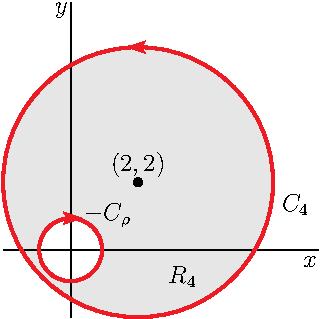
\includegraphics[scale=0.90]{OE16D_4c.pdf}\qquad
\end{center}

(b) We cannot blindly apply Green's theorem to $I_3=\int_{C_3}\vF\cdot\dee{\vr}$
because $(0,0)$ \emph{is} in the interior of $C_3$, so that 
$Q_x-P_y$ is not identically zero in the interior of $C_3$ --- it is not
even defined throughout the interior of $C_3$. We can work around this obstruction by considering the interior of $C_3$ with the interior of $C_1$
removed. That is, by considering
\begin{equation*}
R_3 = \Set{(x,y)}{x^2 + (y - 2)^2 \le 9,\ x^2+y^2\ge 1}
\end{equation*}
It is sketched on the right above.
The boundary of $R_3$ consists of two parts
\begin{itemize}\itemsep1pt \parskip0pt \parsep0pt %\itemindent-15pt
\item[$\circ$]
the circle $C_3$, oriented counterclockwise, and
\item[$\circ$]
the circle $-C_1$. That is, the circle $C_1$ but oriented clockwise,
rather than counterclockwise.
\end{itemize}
Then $Q_x-P_y$ is well-defined and zero throughout $R_3$ and,
by Green's theorem,
\begin{align*}
   0 &=\dblInt_{R_3} \big(Q_x-P_y\big)\,\dee{x}\dee{y} 
     = \int_{C_3} \vF\cdot\dee{\vr} 
             + \int_{-C_1} \vF\cdot\dee{\vr} \\
    &= \int_{C_3} \vF\cdot\dee{\vr} 
             - \int_{C_1} \vF\cdot\dee{\vr} \\
    &= \int_{C_3} \vF\cdot\dee{\vr} 
             - \pi 
\end{align*}
So $\int_{C_3} \vF\cdot\dee{\vr} = \pi$.

(c) Again, we cannot blindly apply Green's theorem 
to $I_4=\int_{C_4}\vF\cdot\dee{\vr}$
because $(0,0)$ \emph{is} in the interior of $C_4$. This time
we cannot remove the interior of $C_1$ from the interior of $C_4$,
because $C_1$ is not contained in the interior of $C_4$. Instead
we pick a number $\rho>0$ which is small enough that the
positively oriented circle 
\begin{equation*}
C_\rho = \Set{(x,y)}{x^2+y^2=\rho^2}
\end{equation*}
is completely inside $C_4$. Then we can define
\begin{equation*}
R_4 = \Set{(x,y)}{(x-2)^2 + (y - 2)^2 \le 9,\ x^2+y^2\ge \rho^2}
\end{equation*}
It is sketched on the left below. We can now argue as in part (b).
The boundary of $R_4$ consists of two parts
\begin{itemize}\itemsep1pt \parskip0pt \parsep0pt %\itemindent-15pt
\item[$\circ$]
the circle $C_4$, oriented counterclockwise, and
\item[$\circ$]
the circle $-C_\rho$. That is, the circle $C_\rho$ but oriented clockwise,
rather than counterclockwise.
\end{itemize}
Then $Q_x-P_y$ is well-defined and zero throughout $R_4$ and,
by Green's theorem,
\begin{align*}
   0 &=\dblInt_{R_4} \big(Q_x-P_y\big)\,\dee{x}\dee{y} \\
    &= \int_{C_4} \vF\cdot\dee{\vr} 
             + \int_{-C_\rho} \vF\cdot\dee{\vr} \\
    &= \int_{C_4} \vF\cdot\dee{\vr} 
             - \int_{C_\rho} \vF\cdot\dee{\vr} 
\end{align*}
So $\int_{C_4} \vF\cdot\dee{\vr} = \int_{C_\rho} \vF\cdot\dee{\vr}$.

To complete our computation, we have to determine 
$\int_{C_\rho} \vF\cdot\dee{\vr}$. We can do so by repeating the
same ``removing a small disk containing $(0,0)$'' argument for the third time.
Set
\begin{equation*}
R_5 = \Set{(x,y)}{x^2 + y^2 \le 1,\ x^2+y^2\ge \rho^2}
\end{equation*}
Then the boundary of $R_5$ consists of $C_1$ and $-C_\rho$,
and, as $Q_x-P_y$ is well-defined and zero throughout $R_5$,
\begin{align*}
   0 &=\dblInt_{R_5} \big(Q_x-P_y\big)\,\dee{x}\dee{y} \\
    &= \int_{C_1} \vF\cdot\dee{\vr} 
             + \int_{-C_\rho} \vF\cdot\dee{\vr} \\
    &= \pi
             - \int_{C_\rho} \vF\cdot\dee{\vr} 
\end{align*}
So $\int_{C_4} \vF\cdot\dee{\vr} = \int_{C_\rho} \vF\cdot\dee{\vr}=\pi$.

\begin{center}
     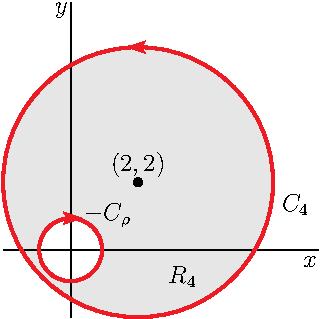
\includegraphics[scale=0.90]{OE16D_4c.pdf}\qquad
     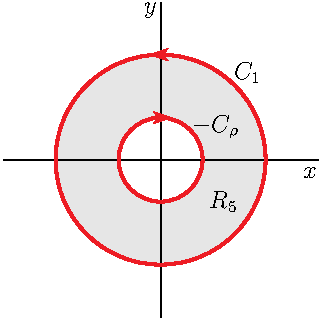
\includegraphics[scale=0.90]{OE16D_4d.pdf}
\end{center}
\end{solution}

%%%%%%%%%%%%%%%%%%%%%%%%%%%
\begin{question}[M317 2017A] %6
Consider the vector field $\vF = P\,\hi + Q\,\hj$, where
\begin{equation*}
P=\frac{x+y}{x^2+y^2},\qquad
Q=\frac{y-x}{x^2+y^2}
\end{equation*}
\begin{enumerate}[(a)]
\item
Compute and simplify $Q_x - P_y$.

\item
Compute the integral $\int_{C_R} \vF \cdot \dee{\vr}$ 
directly using a parameterization, where $C_R$ is the circle of radius $R$, 
centered at the origin, and oriented in the counterclockwise direction.

\item 
Is $\vF$ conservative? Carefully explain how your answer fits with the 
results you got in the first two parts.

\item
Use Green's theorem to compute $\int_C \vF \cdot \dee{\vr}$ where $C$ 
is the triangle with vertices $(1, 1)$, $(1, 0)$, $(0, 1)$ oriented in 
the counterclockwise direction.

\item
Use Green's theorem to compute $\int_C \vF \cdot \dee{\vr}$ where $C$ 
is the triangle with vertices $(-1, -1)$, $(1, 0)$, $(0, 1)$ oriented in 
the counterclockwise direction.

\end{enumerate}
\end{question}

%\begin{hint} 
%\end{hint}

\begin{answer} 
(a) $Q_x-P_y=0$ except at $(0,0)$ where it is not defined.

(b) $-2\pi$\qquad
(c) No.\qquad
(d) $0$\qquad
(e) $-2\pi$
\end{answer}

\begin{solution} (a)  If $(x,y)\ne (0,0)$, we have
\begin{align*}
Q_x - P_y
&=\pdiff{}{x}\Big(\frac{y-x}{x^2+y^2}\Big)
-\pdiff{}{y}\Big(\frac{x+y}{x^2+y^2}\Big) \\
&=\frac{-(x^2+y^2)-(y-x)(2x)}{{(x^2+y^2)}^2}
      -\frac{(x^2+y^2)-(x+y)(2y)}{{(x^2+y^2)}^2}\\
&=0
\end{align*}

(b) Parametrize $C_R$ by
\begin{equation*}
\vr(\theta) = R\cos\theta\,\hi +R\sin\theta\,\hj\qquad
0\le\theta\le 2\pi
\end{equation*}
So
\begin{align*}
\int_{C_R} \vF \cdot \dee{\vr}
&=\int_0^{2\pi} \overbrace{\frac{1}{R}
   \left\{\big(\cos\theta+\sin\theta\big)\hi
           +\big(\sin\theta-\cos\theta\big)\hj\right\}}^{\vF(\vr(\theta))} 
       \cdot
     \big(\overbrace{-R\sin\theta\,\hi+R\cos\theta\,\hj}^{\vr'(\theta)}\big)
           \,\dee{\theta}
\\
&=\int_0^{2\pi}(-1)\ \dee{\theta} \\
&=-2\pi
\end{align*}

(c) If $\vF$ were conservative, the line integral $\int_C\vF\cdot\dee{\vr}$
would be $0$ for any closed curve $C$, by 
Theorem \eref{CLP317}{thm:pathIndepConserv}.b in the CLP-4 text. 
So $\vF$ is \emph{not} conservative. Note that $\vF$ is not defined at
$(x,y) = (0,0)$ and so fails the screening
test $\vnabla\times\vF=\vZero$ at $(x,y)=(0,0)$.

(d) Denote by $\cR$ the interior of the triangle $C$. It is the grey
region in the figure
\begin{center}
     \includegraphics{OE17A_6a}
\end{center}
Note that $(0,0)$ is \emph{not} in $\cR$. So $Q_x - P_y$ is defined
and zero throughout $\cR$. So, by Green's theorem  (Theorem \eref{CLP317}{thm:Green} in the CLP-4 text), 
\begin{align*}
\int_C \vF \cdot \dee{\vr}
&= \dblInt_\cR\big(Q_x - P_y\big)\,\dee{x}\dee{y}
=0
\end{align*}

(e) Note that $(0,0)$ \emph{is} in the interior of triangle $C$ specified 
for this part. So $Q_x - P_y$ is \emph{not} defined in that interior 
and we cannot apply Green's theorem precisely as we did in part (d).
We can work around this obstruction by 
\begin{itemize}\itemsep1pt \parskip0pt \parsep0pt %\itemindent-15pt
\item[$\circ$]
picking a number $r>0$ that is small
enough that the circle $C_r$, of radius $r$ centred on $(0,0)$,
is completely contained in the interior of the triangle $C$. 
\item[$\circ$]
Then we work with
the region $\cR$ defined by removing the interior of the circle $C_r$
from the interior of the triangle $C$. It is the grey region sketched below.
\begin{center}
     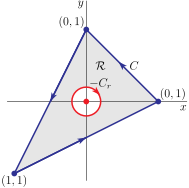
\includegraphics{OE17A_6b}
\end{center}
\end{itemize}
The boundary of $\cR$ consists of two parts
\begin{itemize}\itemsep1pt \parskip0pt \parsep0pt %\itemindent-15pt
\item[$\circ$]
the triangle $C$, oriented counterclockwise, and
\item[$\circ$]
the circle $-C_r$. That is, the circle $C_r$, but oriented clockwise,
rather than counterclockwise.
\end{itemize}
Then $Q_x-P_y$ is well-defined and zero throughout $\cR$ and,
by Green's theorem,
\begin{align*}
   0 &=\dblInt_\cR \big(Q_x-P_y\big)\,\dee{x}\dee{y} \\
    &= \int_C \vF\cdot\dee{\vr} 
             + \int_{-C_r} \vF\cdot\dee{\vr} \\
    &= \int_C \vF\cdot\dee{\vr} 
             - \int_{C_r} \vF\cdot\dee{\vr} 
\end{align*}
So $\int_C \vF\cdot\dee{\vr} = \int_{C_r} \vF\cdot\dee{\vr} $.
By part (b), with $R=r$, $\int_{C_r} \vF\cdot\dee{\vr}=-2\pi$, so
$\int_C \vF\cdot\dee{\vr} = -2\pi$
\end{solution}

%%%%%%%%%%%%%%%%%%%%%%%%%%%%%%%
\begin{question}[M317 2017D] %7
\begin{enumerate}[(a)]
\item
Evaluate
\begin{equation*}
\int_C \sqrt{1+x^3}\,\dee{x} +\big(2xy^2 + y^2\big)\,\dee{y}
\end{equation*}
where $C$ is the unit circle $x^2+y^2 = 1$, oriented counterclockwise.

\item 
Evaluate
\begin{equation*}
\int_C \sqrt{1+x^3}\,\dee{x} +\big(2xy^2 + y^2\big)\,\dee{y}
\end{equation*}
where $C$ is now the part of the unit circle $x^2+y^2 = 1$, with $x\ge 0$, 
still oriented counterclockwise.
\end{enumerate}
\end{question}

%\begin{hint} 
%\end{hint}

\begin{answer} 
(a) $\frac{\pi}{2}$\qquad
(b) $\frac{\pi}{4}+\frac{2}{3}$
\end{answer}

\begin{solution} (a) The given integral is of the form 
  $\int_C F_1(x,y)\,\dee{x}+F_2(x,y)\,\dee{y}$ with
\begin{equation*}
F_1(x,y) = \sqrt{1+x^3}\qquad
F_2(x,y) = 2xy^2 + y^2\qquad
\frac{\partial F_2}{\partial x} - \frac{\partial F_1}{\partial y} = 2y^2
\end{equation*}
As $C$ is $\partial R$ with 
\begin{equation*}
R = \Set{(x,y)}{ x^2+y^2\le 1}
\end{equation*}
Green's theorem (Theorem \eref{CLP317}{thm:Green} in the CLP-4 text)
gives
\begin{align*}
\int_C \sqrt{1+x^3}\,\dee{x} +\big(2xy^2 + y^2\big)\,\dee{y}
& = \int_C F_1(x,y)\,\dee{x}+F_2(x,y)\,\dee{y}
  = \dblInt_R \Big(\frac{\partial F_2}{\partial x} 
           - \frac{\partial F_1}{\partial y}\Big)\ \dee{x}\dee{y} \\
&= 2 \dblInt_R y^2\ \dee{x}\dee{y}
\end{align*}
Switching to polar coordinates
\begin{align*}
\int_C \sqrt{1+x^3}\,\dee{x} +\big(2xy^2 + y^2\big)\,\dee{y}
&= 2\int_0^{2\pi}\dee{\theta} \int_0^1\dee{r}\ 
         r\big(r\sin\theta\big)^2 \\
&= 2\left[\int_0^{2\pi}\dee{\theta}\ \sin^2\theta\right]
   \left[\int_0^1\dee{r}\ r^3\right]
=2\ \pi\ \frac{1}{4}
=\frac{\pi}{2}
\end{align*}
To do the $\theta$ integral, we have used
\begin{align*}
\int_0^{2\pi} \sin^2 \theta\ \dee{\theta}
=\int_0^{2\pi} \Big(\frac{1-\cos(2\theta)}{2}\Big)\,\dee{\theta}  
=\Big[\frac{\theta-\sin(2\theta)/2}{2} \Big]_0^{2\pi} 
= \pi
\end{align*}
For an efficient, sneaky, way to evaluate 
$\int_0^{2\pi} \sin^2 \theta\ \dee{\theta}$, see Example
\eref{CLP317}{eg:workIntegalB} in the CLP-4 text.

(b) It is again natural to use Green's theorem.
But Green's theorem must be applied to a curve that is closed,
so that it is the boundary of a region in $\bbbr^2$. The given curve $C$
is not closed. But it is  part of the boundary of 
\begin{equation*}
R = \Set{(x,y)}{x^2+y^2\le 1,\ x\ge 0}
\end{equation*}
Here is a sketch of $R$.
 \begin{center}
    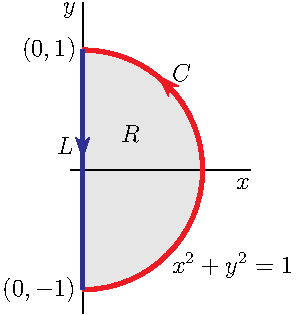
\includegraphics{OE17D_7.pdf}
\end{center}

The boundary of $R$ consists of two parts --- $C$ on the right
and the line segment $L$ from $(0,1)$ to $(0,-1)$ on the left.
Note that $\vF=F_1\,\hi +F_2\,\hj$ is well-defined on all of $R$ 
and that we still have, from part (a),
\begin{align*}
\frac{\partial F_2}{\partial x}  - 
\frac{\partial F_1}{\partial y} 
&=2y^2
\end{align*}
on all of $R$. So, by Green's theorem (Theorem \eref{CLP317}{thm:Green} in the CLP-4 text), 
\begin{align*}
\int_C \sqrt{1+x^3}\,\dee{x} +\big(2xy^2 + y^2\big)\,\dee{y}
&=\dblInt_R \Big(\frac{\partial F_2}{\partial x} - 
          \frac{\partial F_2}{\partial y} \Big)\dee{x}\dee{y}
 - \int_L\vF\cdot\dee{\vr} \\
&=\dblInt_{\Atop{x^2+y^2\le 1}{x\ge 0}} 2y^2\  \dee{x}\dee{y}
  + \int_{-L} F_2\,\dee{y} \\
&=\dblInt_{x^2+y^2\le 1} y^2\  \dee{x}\dee{y}
  + \int_{-1}^1 y^2\,\dee{y} \\
&\hskip0.25in\text{by symmetry for the first integral and} \\
&\hskip0.25in\text{since $x=0$ and $\dee{x}=0$ in the second integral} \\
&=\frac{\pi}{4} + \frac{2}{3}
\end{align*}
In the second line, we used the notation $-L$ for the line segment
from $(0,-1)$ to $(0,1)$.
\end{solution}





%%%%%%%%%%%%%%%%%%
\subsection*{\Application}
%%%%%%%%%%%%%%%%%%


%%%%%%%%%%%%%%%%%%%%%%%%%%%
\begin{question}[M317 2007A] %6
Evaluate the line integral
\begin{equation*}
\int_C (x^2 + y e^x ) \,\dee{x} + (x \cos y + e^x ) \,\dee{y}
\end{equation*}
where $C$ is the arc of the curve $x = \cos y$ for $-\pi/2 \le y \le \pi/2$, 
traversed in the direction of increasing $y$.
\end{question}

\begin{hint} 
It is possible to evaluate this integral by three different methods,
one of them being direct evaluation (though it requires
some ingenuity). Try to find all three.
\end{hint}

\begin{answer} 
$\frac{3\pi}{2}$
\end{answer}

\begin{solution} 
First, here is a sketch of the curve $C$.

     \begin{center}
          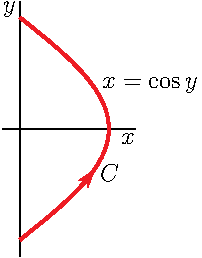
\includegraphics{OE07A_6.pdf}
     \end{center}


We'll evaluate this integral in three different ways.
\begin{enumerate}[(1)]
\item \emph{Direct evaluation:}\ \ \ To evaluate the integral directly,
we'll parametrize $C$ using $y$ as the parameter. That is, we'll make $y(t)=t$:
\begin{align*}
\vr(t) &= x(t)\,\hi+y(t)\,\hj
        = \cos t\,\hi + t\,\hj\qquad -\frac{\pi}{2}\le t\le\frac{\pi}{2} \\
\vr'(t) &= x'(t)\,\hi+y'(t)\,\hj
        = -\sin t\,\hi + \hj 
\end{align*}
So the integral is
\begin{align*}
&\int_C (x^2 + y e^x ) \,\dee{x} + (x \cos y + e^x ) \,\dee{y} \\
&\hskip0.5in
  =\int_{-\pi/2}^{\pi/2}\Big\{ \big[x(t)^2 +y(t) e^{x(t)}\big]\diff{x}{t}(t)
                        +  \big[x(t) \cos(y(t)) + e^{x(t)}\big]\diff{y}{t}(t)
                        \Big\}\dee{t} \\
&\hskip0.5in
  =\int_{-\pi/2}^{\pi/2}\Big\{ -\big[\cos^2 t + t e^{\cos t}\big]\sin t
                           +  \big[\cos^2 t + e^{\cos t}\big]
                        \Big\}\dee{t} \\
&\hskip0.5in
  =\int_{-\pi/2}^{\pi/2}\Big\{ -\cos^2 t\sin t +\cos^2 t 
                      - t e^{\cos t}\sin t + e^{\cos t}
                        \Big\}\dee{t} \\
&\hskip0.5in
  =\int_{-\pi/2}^{\pi/2}\Big\{ \cos^2 t 
                  +\diff{\hfill}{t}\Big[\frac{\cos^3 t}{3} +te^{\cos t}\Big]
                        \Big\}\dee{t} \\
&\hskip0.5in
  =\int_{-\pi/2}^{\pi/2}\Big\{ \frac{\cos(2t)+1}{2}
                  +\diff{\hfill}{t}\Big[\frac{\cos^3 t}{3} +te^{\cos t}\Big]
                        \Big\}\dee{t} \\
&\hskip0.5in
  =\Big[ \frac{\sin(2t)}{4} +\frac{t}{2}+
                  \frac{\cos^3 t}{3} +te^{\cos t}
                        \Big]_{-\pi/2}^{\pi/2} \\
&\hskip0.5in
  =\frac{3\pi}{2}
\end{align*}
For an efficient, sneaky, way to evaluate 
$\int_{-\pi/2}^{\pi/2} \cos^2 t\ \dee{t}$ see Example
\eref{CLP317}{eg:workIntegalB} in the CLP-4 text.

\item \emph{Green's (or Stokes') theorem:}
The curve $C$ is not closed so we cannot apply Green's theorem directly.
However the boundary of the region
\begin{equation*}
R = \Set{(x,y)}{ 0\le x\le\cos y,\ 
           -\nicefrac{\pi}{2}\le y\le \nicefrac{\pi}{2} }
\end{equation*}
(sketched below) consists of two parts, one of which is $C$. The other 
is the line $L$ from $\big(0,\nicefrac{\pi}{2}\big)$ 
to $\big(0,-\nicefrac{\pi}{2}\big)$.

     \begin{center}
          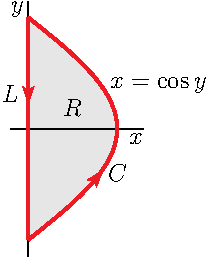
\includegraphics{OE07A_6b.pdf}
     \end{center}

So Green's theorem gives
\begin{align*}
&\int_C (x^2 + y e^x ) \,\dee{x} + (x \cos y + e^x ) \,\dee{y} \\
&\hskip0.25in=\dblInt_R \Big\{\pdiff{}{x}(x \cos y + e^x )
          -\pdiff{}{y}(x^2 + y e^x )\Big\}\dee{x}\dee{y}
-\int_L (x^2 + y e^x ) \,\dee{x} + (x \cos y + e^x ) \,\dee{y} \\
&\hskip0.25in=\dblInt_R \cos y\ \dee{x}\dee{y}  -  \int_L \,\dee{y}\qquad
    \text{since $x=0$ and $\dee{x}=0$ on $L$} \\
&\hskip0.25in=\int_{-\pi/2}^{\pi/2}\dee{y}\int_0^{\cos y}\dee{x}\ \cos y
                       -\int_{\pi/2}^{-\pi/2}\dee{y} \\
&\hskip0.25in=\int_{-\pi/2}^{\pi/2}\dee{y}\ \cos^2 y
                       + \pi \\
&\hskip0.25in
  =\int_{-\pi/2}^{\pi/2} \frac{\cos(2y)+1}{2}\ \dee{y} + \pi \\
&\hskip0.25in
  =\Big[ \frac{\sin(2y)}{4} +\frac{y}{2}\Big]_{-\pi/2}^{\pi/2} +\pi \\
&\hskip0.25in
  =\frac{3\pi}{2}
\end{align*}


\item \emph{(Sort of) conservative fields:}\ \ \ The given integral
is $\int_C\vF\cdot\dee{\vr}$ with 
$\vF = (x^2 + y e^x ) \,\hi + (x \cos y + e^x ) \,\hj$. The curl of this
field is
\begin{align*}
\vnabla\times\vF
&=\det\left[\begin{matrix}
\hi &\hj &\hk \\
\tfrac{\partial\hfill}{\partial x} & \tfrac{\partial\hfill}{\partial y} & 
                \tfrac{\partial\hfill}{\partial z} \\
x^2 + y e^x & x \cos y + e^x & 0
\end{matrix}
\right]
=\cos y\,\hk
\end{align*}
So $\vF$ violates our screening test and consequently is not conservative.
But it violates the screening test only because of the term $x\cos y\,\hj$.
This suggests that we split up 
\begin{equation*}
\vF = \vG +\vH\qquad\text{with}\quad
\vG= (x^2 + y e^x ) \,\hi + e^x \,\hj,\quad
\vH = x\cos y\,\hj
\end{equation*}
Then $\vG$ is conservative with potential $g=\frac{x^3}{3}+ye^x$
and $\vH$ is pretty simple, so that it is not hard to evaluate 
$\int_C\vH\cdot\dee{\vr}$ directly. Using the parametrization 
$\vr(t) = \cos t\,\hi + t\,\hj$,  $-\frac{\pi}{2}\le t\le\frac{\pi}{2}$
as above,
\begin{align*}
\int_C\vF\cdot\dee{\vr}
&= \int_C\vG\cdot\dee{\vr} + \int_C\vH\cdot\dee{\vr} \\
&= \int_C\vnabla g\cdot\dee{\vr} + \int_C\vH\cdot\dee{\vr} \\
&=g\big(\vr(\nicefrac{\pi}{2})\big) -g\big(\vr(-\nicefrac{\pi}{2})\big)
   + \int_{-\pi/2}^{\pi/2} x(t) \cos(y(t)) \diff{y}{t}(t)\ \dee{t} \\
& =g\big(0,\nicefrac{\pi}{2}\big) -g\big(0,-\nicefrac{\pi}{2}\big)
   +\int_{-\pi/2}^{\pi/2} \cos^2 t \,\dee{t} \\
&=\frac{\pi}{2} -\Big(-\frac{\pi}{2}\Big)
   +\int_{-\pi/2}^{\pi/2} \frac{\cos(2t)+1}{2} \dee{t} \\
&=\pi  + \Big[ \frac{\sin(2t)}{4} +\frac{t}{2}\Big]_{-\pi/2}^{\pi/2} \\
&=\frac{3\pi}{2}
\end{align*}

\end{enumerate}

\end{solution}

%%%%%%%%%%%%%%%%%%%%%%%%%%%
\begin{question}[M317 2004A] %5
 Use Green's theorem to establish that if $C$ is a simple
closed curve in the plane, then the area $A$ enclosed by $C$ is given by
\begin{equation*}
A=\frac{1}{2}\oint_C x\,\dee{y}-y\,\dee{x}
\end{equation*}
Use this to calculate the area inside the curve 
$x^{2/3}+y^{2/3}=1$.
\end{question}

%\begin{hint} 
%\end{hint}

\begin{answer} 
$\frac{3\pi}{8}$
\end{answer}

\begin{solution} 
Call the region enclosed by the curve $R$. By Green's theorem,
Theorem \eref{CLP317}{thm:Green} in the CLP-4 text,
\begin{equation*}
\frac{1}{2}\oint_C x\,\dee{y}-y\,\dee{x}
=\frac{1}{2}\dblInt_R\Big(\pdiff{}{x}x
-\pdiff{}{y}(-y)\Big)\ \dee{x}\dee{y}
=\frac{1}{2}\dblInt_R 2\ \dee{x}\dee{y}
=A
\end{equation*}
as desired. The curve $x^{2/3}+y^{2/3}=1$ may be parametrized in the 
counterclockwise orientation by $x(\theta)=\cos^3\theta$, $y(\theta)=\sin^3\theta$,
$0\le\theta\le 2\pi$. Then
\begin{align*}
A&=\frac{1}{2}\oint_C x\,\dee{y}-y\,\dee{x} \\
&=\frac{1}{2}\int_0^{2\pi}\big( x(\theta)y'(\theta)-y(\theta)x'(\theta)\big)\ \dee{\theta}
=\frac{1}{2}\int_0^{2\pi}\big( 3\cos^4\theta\sin^2\theta+3\sin^4\theta\cos^2\theta\big)\ \dee{\theta}\\
&=\frac{3}{2}\int_0^{2\pi}\sin^2\theta\cos^2\theta\ \dee{\theta}
=\frac{3}{8}\int_0^{2\pi}\sin^2(2\theta)\ \dee{\theta} \\
&=\frac{3}{16}\int_0^{2\pi}\big(1-\cos(4\theta)\big)\ \dee{\theta}
=\frac{3}{16}\Big[\theta-\frac{1}{4}\sin(4\theta)\Big]_0^{2\pi}
=\frac{3\pi}{8}
\end{align*}
\end{solution}

%%%%%%%%%%%%%%%%%%%%%%%%%%%
\begin{question}[M317 2001D] %3
Let $\vF(x,y)=(x+3y)\,\hi+(x+y)\,\hj$ and 
$\vG(x,y)=(x+y)\,\hi+(2x-3y)\,\hj$ be vector fields. Find a number $A$ such
that for each circle $C$ in the plane
$$
\oint_C\vF\cdot \dee{\vr}=A\oint_C\vG\cdot \dee{\vr}
$$
\end{question}

\begin{hint} 
Write $\oint_C\vF\cdot \dee{\vr}-A\oint_C\vG\cdot \dee{\vr}
=\oint_C(\vF-A\vG)\cdot \dee{\vr}$.
\end{hint}

\begin{answer} 
$A=-2$
\end{answer}

\begin{solution} 
If we use $D$ to denote the disk inside the circle $C$
then we want
$$
\oint_C\vF\cdot \dee{\vr}-A\oint_C\vG\cdot \dee{\vr}
=\oint_C(\vF-A\vG)\cdot \dee{\vr}
=\dblInt_D \Big[\pdiff{}{x}(\vF-A\vG)_2
-\pdiff{}{y}(\vF-A\vG)_1\Big]\,\dee{x}\dee{y}
$$
to vanish for all disks $D$. We used Green's theorem, which is Theorem
\eref{CLP317}{thm:Green} in the CLP-4 text,  in the last step. 
This is the case if and only if
\begin{align*}
&\pdiff{}{x}(\vF-A\vG)_2
=\pdiff{}{y}(\vF-A\vG)_1\\
\iff&
\pdiff{}{x}[(x+y)-A(2x-3y)]
=\pdiff{}{y}[(x+3y)-A(x+y)]\\
\iff&
1-2A=3-A\\
\iff& A=-2
\end{align*}
\end{solution}

%%%%%%%%%%%%%%%%%%%%%%%%%%%
\begin{question}[M317 2001D] %6
Let
$\vF(x,y) = \frac{y^3}{ {(x^2+y^2)}^2}\hi
              -\frac{xy^2}{ {(x^2+y^2)}^2}\hj$, $(x,y)\ne (0,0)$.
\smallskip
\begin{enumerate}[(a)]
\item 
Compute $\oint_C\vF\cdot \dee{\vr}$ where $C$ is the unit circle
in the $xy$-plane, positively oriented.

\item
Use (a) and Green's theorem to find $\oint_{C_0}\vF\cdot \dee{\vr}$
where $C_0$ is the ellipse $\frac{x^2}{16}+\frac{y^2}{25}=1$, positively
oriented.

\end{enumerate}
\end{question}

\begin{hint} 
Note that $\vF(x,y)$ is not defined at $(x,y)=(0,0)$.
\end{hint}

\begin{answer} 
$-\pi$
\end{answer}

\begin{solution} 
(a) Parametrize the circle $\vr(\theta)=(\cos\theta,\sin\theta)$. Then
\begin{align*}
\vF\big(\vr(\theta)\big)
&=\sin^3\theta\,\hi -\cos\theta \sin^2\theta\,\hj\\
\diff{\vr}{\theta}(\theta)&=-\sin\theta\,\hi+\cos\theta\,\hj\\
\vF\big(\vr(\theta)\big)\cdot \diff{\vr}{\theta}(\theta)
&=-\sin^4\theta-\cos^2\theta\sin^2\theta=-\sin^2\theta\\
\oint_C\vF\cdot \dee{\vr}
&=\int_0^{2\pi}\vF\big(\vr(\theta)\big)\cdot \diff{\vr}{\theta}(\theta)\ \dee{\theta}
=-\int_0^{2\pi}\sin^2\theta\ \dee{\theta}
=-\int_0^{2\pi}\frac{1-\cos(2\theta)}{2}\ \dee{\theta}\\
&=-{\Big[\frac{\theta}{2}-\frac{\sin(2\theta)}{4}\Big]}_0^{2\pi}
=-\pi
\end{align*}
For an efficient, sneaky, way to evaluate 
$\int_0^{2\pi} \sin^2\theta\ \dee{\theta}$ see Example
\eref{CLP317}{eg:workIntegalB} in the CLP-4 text.

(b) Denote by $W$ the washer shaped region between the circle
$x^2+y^2=1$ and the ellipse $\frac{x^2}{16}+\frac{y^2}{25}=1$. 
It is sketched below. By Green's theorem
\begin{align*}
\oint_{C_0}\vF\cdot \dee{\vr}-\oint_C\vF\cdot \dee{\vr}
=\dblInt_W \Big[\pdiff{}{x}\vF_2
-\pdiff{}{y}\vF_1\Big]\,\dee{x}\dee{y}
\end{align*}
For the specified $\vF$
\begin{align*}
\pdiff{}{x}\vF_2
-\pdiff{}{y}\vF_1
&=-\pdiff{}{x}\frac{xy^2}{ {(x^2+y^2)}^2}
-\pdiff{}{y}\frac{y^3}{ {(x^2+y^2)}^2}\\
&=-\frac{y^2}{ {(x^2+y^2)}^2}+2\frac{xy^2(2x)}{ {(x^2+y^2)}^3}
-\frac{3y^2}{ {(x^2+y^2)}^2}+2\frac{y^3(2y)}{ {(x^2+y^2)}^3}\\
&=\frac{-y^2(x^2+y^2)+4x^2y^2-3y^2(x^2+y^2)+4y^4}{ {(x^2+y^2)}^3}\\
&=0
\end{align*}
Consequently
$$
\oint_{C_0}\vF\cdot \dee{\vr}-\oint_C\vF\cdot \dee{\vr}=0
\implies
\oint_{C_0}\vF\cdot \dee{\vr}=\oint_C\vF\cdot \dee{\vr}=-\pi
$$

\begin{center}
   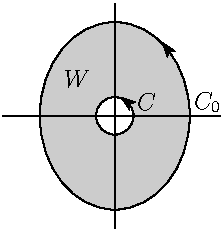
\includegraphics{OE01DQ6.pdf}
\end{center}

\end{solution}

%%%%%%%%%%%%%%%%%%%%%%%%%%%
\begin{question}[M317 2001A] %5
Let $\cC_1$ be the circle $(x-2)^2+y^2=1$ and let $\cC_2$ be
the circle $(x-2)^2+y^2=9$. Let 
$\vF=-\frac{y}{x^2+y^2}\,\hi+\frac{x}{x^2+y^2}\,\hj$. Find the integrals
$\oint_{\cC_1}\vF\cdot \dee{\vr}$ and $\oint_{\cC_2}\vF\cdot \dee{\vr}$.
\end{question}

\begin{hint} 
Note that $\vF(x,y)$ is not defined at $(x,y)=(0,0)$.
\end{hint}

\begin{answer} 
$\oint_{\cC_1}\vF\cdot \dee{\vr}=0$ and $\oint_{\cC_2}\vF\cdot \dee{\vr}=2\pi$
\end{answer}

\begin{solution} 
Observe that
\begin{align*}
\frac{\partial F_2}{\partial x}
-\frac{\partial F_1}{\partial y}
&=\frac{\partial \hfill}{\partial x}\Big( \frac{x}{x^2+y^2}\Big)
-\frac{\partial \hfill}{\partial y}\Big( \frac{-y}{x^2+y^2}\Big)\\
&=\frac{(x^2+y^2)-x(2x)}{{(x^2+y^2)}^2}
+\frac{(x^2+y^2)-y(2y)}{{(x^2+y^2)}^2}=0
\end{align*}
except at $(0,0)$, where $\vF$ is not defined. Hence by Green's theorem
(Theorem \eref{CLP317}{thm:Green} in the CLP-4 text),
$\oint_{\cC}\vF\cdot \dee{\vr}=0$ for any closed curve that does not contain
$(0,0)$ in its interior. 
In particular, $\oint_{\cC_1}\vF\cdot \dee{\vr}=0$. On the other hand,
$(0,0)$ is contained in the interior of $\cC_2$, so we cannot use
Green's theorem to conclude that $\oint_{\cC_2}\vF\cdot \dee{\vr}=0$.

Let $\cC_3$ be the circle of radius one centred on $(0,0)$ and
denote by $W$ the washer shaped region between the circle
$\cC_2$ and the circle $\cC_3$. It is sketched below.

\begin{center}
   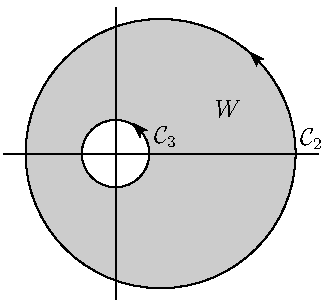
\includegraphics{OE01AQ5.pdf}
\end{center}

 By Green's theorem (Theorem \eref{CLP317}{thm:Green} in the CLP-4 text),
\begin{align*}
\oint_{\cC_2}\vF\cdot \dee{\vr}-\oint_{\cC_3}\vF\cdot \dee{\vr}
=\dblInt_W \Big[\pdiff{}{x}\vF_2
-\pdiff{}{y}\vF_1\Big]\,\dee{x}\dee{y}
=0
\end{align*} 
So
$\oint_{\cC_2}\vF\cdot \dee{\vr}=\oint_{\cC_3}\vF\cdot \dee{\vr}$. Parameterize
$\cC_3$ by $x=\cos\theta$, $y=\sin\theta$. Then
\begin{align*}
\vr(\theta)&=\cos\theta\,\hi+\sin\theta\,\hj\qquad 0\le \theta\le 2\pi\\
\vr'(\theta)&=-\sin\theta\,\hi+\cos\theta\,\hj\\
\vF\big(\vr(\theta)\big)&=-\sin\theta\,\hi+\cos\theta\,\hj\\
\vF\big(\vr(\theta)\big)\cdot\vr'(\theta)
&=1\\
\end{align*}
so that
$$
\oint_{\cC_2}\vF\cdot \dee{\vr}
=\oint_{\cC_3}\vF\cdot \dee{\vr}
=\int_0^{2\pi} \dee{\theta}\ 1
=2\pi
$$
\end{solution}

%%%%%%%%%%%%%%%%%%%%%%%%%%%
\begin{question}[M317 2000A] %3
Let $R$ be the region in the first quadrant of the $xy$-plane
bounded by the coordinate axes and the curve $y=1-x^2$. Let $\cC$ be the
boundary of $R$, oriented counterclockwise.
\begin{enumerate}[(a)]
\item
Evaluate $\int_\cC x\,\dee{s}$.
\item
 Evaluate $\int_\cC \vF\cdot \dee{\vr}$, where $\vF(x,y)
=\big(\sin(x^2)-xy\big)\,\hi+\big(x^2+\cos(y^2)\big)\,\hj$.
\end{enumerate}
\end{question}

%\begin{hint} 
%\end{hint}

\begin{answer} 
(a) $\frac{1}{2}+\frac{1}{12}\big[5^{3/2}-1\big]\approx 1.3484$\qquad
(b) $\frac{3}{4}$
\end{answer}

\begin{solution} 
(a) Let $\cC_1$ be the line segment from $(0,1)$ to $(0,0)$,
$\cC_2$ be the line segment from $(0,0)$ to $(1,0)$ and
$\cC_3$ be the curve $y=1-x^2$ from $(1,0)$ to $(0,1)$.

\begin{center}
   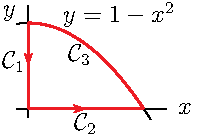
\includegraphics{OE00AQ3.pdf}
\end{center}


 Then
\begin{align*}
\int_{\cC_1} x\,\dee{s}&=\int_{\cC_1} 0\,\dee{s}=0\\
\int_{\cC_2} x\,\dee{s}&=\int_0^1 x\,\dee{x}=\frac{1}{2}
\end{align*}
On $\cC_3$, $y=1-x^2$ so that $\diff{y}{x}=-2x$ and
\begin{equation*}
\dee{s} =\sqrt{\dee{x}^2+\dee{y}^2}
        =\sqrt{1+\Big(\diff{y}{x}\Big)^2}\,\dee{x}
        =\sqrt{1+4x^2}\,\dee{x}
\end{equation*}
and
\begin{align*}
\int_{\cC_3} x\,\dee{s}
&%=\int_1^0 x\sqrt{1+\Big(\diff{y}{x}\Big)^2}\,(-\dee{x})
=\int_0^1 x\sqrt{1+4x^2}\,\dee{x}\\
&=\Big[\frac{1}{12}(1+4x^2)^{3/2}\Big]_0^1
=\frac{1}{12}\big[5^{3/2}-1\big]
\end{align*}
All together
$$
\int_{\cC} x\,\dee{s}=\frac{1}{2}+\frac{1}{12}\big[5^{3/2}-1\big]
\approx 1.3484
$$

(b) By either Stokes' theorem or Green's theorem
\begin{align*}
\int_\cC \vF\cdot \dee{\vr}
&=\dblInt_R\Big[\pdiff{}{x}\big(x^2+\cos(y^2)\big)
-\pdiff{}{y}\big(\sin(x^2)-xy\big) \Big]\ \dee{x} \dee{y}
=\dblInt_R3x\ \dee{x} \dee{y}\\
&=3\int_0^1 \dee{x}\int_0^{1-x^2}\dee{y}\ x
=3\int_0^1 \dee{x}\ (1-x^2) x
=3\Big[\frac{1}{2}-\frac{1}{4}\Big]=\frac{3}{4}
\end{align*}
\end{solution}


%%%%%%%%%%%%%%%%%%%%%%%%%%%
\begin{question}[M317 2010A] %6
Let $C$ be the curve defined by the intersection of the surfaces 
$z = x + y$ and $z = x^2 + y^2$.
\begin{enumerate}[(a)]
\item
Show that $C$ is a simple closed curve.
\item
Evaluate $\oint_C \vF \cdot \dee{\vr}$ where
\begin{enumerate}[(i)]
\item
 $\vF = x^2\,\hi + y^2\,\hj + 3 e^z\,\hk$.
\item 
  $\vF = y^2\,\hi + x^2\,\hj + 3 e^z\,\hk$.
\end{enumerate}
\end{enumerate}
\end{question}

\begin{hint} 
(a) All points on the curve obey an equation that contains $x$'s and $y$'s,
but no $z$'s.

(b) Exploit conservativeness as much as possible.
\end{hint}

\begin{answer} 
(a) The projection of the curve on the $xy$-plane (i.e. the top view of the curve) is a circle. See the solution for more details.

(b) (i) $0$\qquad
(b) (ii) $0$
\end{answer}

\begin{solution} (a)
If $(x,y,z)$ is on the curve, it must obey both $z=x+y$
and $z=x^2+y^2$ and hence it must also obey $x^2+y^2=x+y$
or $(x-\nicefrac{1}{2})^2 + (y-\nicefrac{1}{2})^2 = \nicefrac{1}{2}$.
That's a circle. We can parametrize the curve by
\begin{align*}
x(\theta)&= \frac{1}{2} +\frac{1}{\sqrt{2}}\cos\theta \\
y(\theta)&= \frac{1}{2} +\frac{1}{\sqrt{2}}\sin\theta \\
z(\theta)&= x+y = 1+ \frac{1}{\sqrt{2}}\big[\cos\theta+\sin\theta\big] 
\end{align*}
with $0\le\theta<2\pi$. As $\theta$ runs from $0$ to $2\pi$,
$\big(x(\theta),y(\theta)\big)$ runs once around the circle without
crossing itself so that  $\big(x(\theta),y(\theta),z(\theta)\big)$ runs 
once around the curve without crossing itself. As 
$\big(x(2\pi),y(2\pi),z(2\pi)\big)=\big(x(0),y(0),z(0)\big)$, 
$C$ is a simple closed curve. 

\noindent (b) (i) The vector field $\vF= x^2\,\hi + y^2\,\hj + 3 e^z\,\hk$
is conservative (with potential $\frac{1}{3}x^3 +\frac{1}{3}y^3 + 3e^z$).
So $\oint_C\vF\cdot\dee{\vr}=0$.


\noindent (b) (ii) Note that the question did not specify the orientation
of $C$. It should have. We'll stick with the most commonly used orientation ---
counterclockwise when viewed from high on the $z$-axis.
The vector field $\vG= 3 e^z\,\hk$
is conservative (with potential $3e^z$).
So $\oint_C\vG\cdot\dee{\vr}=0$ and, using the parametrization 
\begin{align*}
\vr(\theta) &= \Big[\frac{1}{2} +\frac{1}{\sqrt{2}}\cos\theta\Big]\hi 
             +\Big[\frac{1}{2} +\frac{1}{\sqrt{2}}\sin\theta\Big]\hj
             +\Big[1 +\frac{1}{\sqrt{2}}\sin\theta
                     +\frac{1}{\sqrt{2}}\cos\theta\Big]\hk \\
\vr'(\theta) &= -\frac{1}{\sqrt{2}}\sin\theta\,\hi 
                +\frac{1}{\sqrt{2}}\cos\theta\,\hj
             +\Big[\frac{1}{\sqrt{2}}\cos\theta
                     -\frac{1}{\sqrt{2}}\sin\theta\Big]\hk
\end{align*}
of part (a), we have
\begin{align*}
\oint_C\vF\cdot\dee{\vr}
&= \oint_C(\vF-\vG)\cdot\dee{\vr} \\
&= \int_0^{2\pi} \big[y(\theta)^2x'(\theta) +x(\theta)^2y'(\theta)\big]
           \dee{\theta} \\
&= \int_0^{2\pi} \Big\{-\Big[\frac{1}{2} +\frac{1}{\sqrt{2}}\sin\theta\Big]^2
                               \frac{1}{\sqrt{2}}\sin\theta
                       +\Big[\frac{1}{2} +\frac{1}{\sqrt{2}}\cos\theta\Big]^2
                               \frac{1}{\sqrt{2}}\cos\theta\Big\}
           \dee{\theta} 
\end{align*}
Because the integral of any odd power of $\sin\theta$ or $\cos\theta$
over $0\le\theta\le 2\pi$ is zero (see Example \eref{CLP317}{eg:stokesD}
in the  text),
\begin{align*}
\oint_c\vF\cdot\dee{\vr}
&= \int_0^{2\pi} \Big\{-\frac{1}{2} \sin^2\theta
                       +\frac{1}{2} \cos^2\theta\Big\}
           \dee{\theta} \\
&=0
\end{align*}
since  (see Example \eref{CLP317}{eg:workIntegalB} in the  text)
\begin{equation*}
\int_0^{2\pi}\cos^2\theta\ \dee{\theta}
=\int_0^{2\pi}\sin^2\theta\ \dee{\theta}
=\pi
\end{equation*}
\end{solution}

%%%%%%%%%%%%%%%%%%%%%%%%%%%
\begin{question}
 Find a smooth, simple, closed, 
counterclockwise oriented curve, $C$, in the $xy$-plane for the which 
the value of the line integral
 $\oint_C(y^3-y)\,\dee{x}-2x^3\,dy$ is a maximum among all 
smooth, simple, closed, counterclockwise oriented curves. 
\end{question}

\begin{hint}
Use Green's theorem to convert the integral over $C$ into an integral 
over the region $R$ in the $xy$-plane whose boundary is $C$. Consider 
the sign of the integrand of the integral over $R$. 
\end{hint}

\begin{answer} 
$6x^2+3y^2= 1$
\end{answer}

\begin{solution} 
By Green's Theorem
\begin{equation*}
\oint_C(y^3-y)\,\dee{x}-2x^3\,\dee{y}
=\dblInt_R\Big[\pdiff{}{x}(-2x^3)
-\pdiff{}{y}(y^3-y)\Big]\ \dee{x}\,\dee{y}
=\dblInt_R\Big[1-6x^2-3y^2\Big]\ \dee{x}\,\dee{y}
\end{equation*}
where $R$ is the region in the $xy$-plane whose boundary is $C$. Observe
that the integrand $1-6x^2-3y^2$ is positive in the elliptical region
 $6x^2+3y^2\le 1$ and negative outside of it. To maximize the integral
$\dblInt_R\big[1-6x^2-3y^2\big]\ \dee{x}\,\dee{y}$ we should choose $R$ to contain
all points $(x,y)$ with the integrand $1-6x^2-3y^2\ge 0$ and to exclude
all points $(x,y)$ with the integrand $1-6x^2-3y^2< 0$. So we
choose 
\begin{equation*}
R=\Set{(x,y)}{6x^2+3y^2\le 1}
\end{equation*}
The corresponding $C$ is $6x^2+3y^2= 1$.



\end{solution}


